
\documentclass{beamer}

\usetheme{Blackboard}

%%%%%%%%%%%%%%%%%%%%%%%%%%%%%%%%%%%%%%%%%%%%%%%%%%
%%%%%%%%%%%%%%%%%%%%%%%%%%%%%%%%%%%%%%%%%%%%%%%%%%
%%%%%%%%%%%%%%%%%%%%%%%%%%%%%%%%%%%%%%%%%%%%%%%%%%
% 各种线条,老熟人无需赘述。
\usepackage{ulem}
%%%%%%%%%%%%%%%%%%%%%%%%%%%%%%%%%%%%%%%%%%%%%%%%%%
%%%%%%%%%%%%%%%%%%%%%%%%%%%%%%%%%%%%%%%%%%%%%%%%%%
%%%%%%%%%%%%%%%%%%%%%%%%%%%%%%%%%%%%%%%%%%%%%%%%%%



\usepackage{mathpazo}

%\usepackage[latin1]{inputenc}
\usepackage[utf8x]{inputenc}
\usepackage[portuguese]{babel}
\usepackage[T1]{fontenc}

\usepackage{subfigure}

%%%%%%%%%%%%%%%%%%%%%%%%%%%%%%%%%%%%%%%%%%%%%%%%%%
%packages para usar letras gregas em negrito
\usepackage{bm} %opcao 2
%$\hat{\bm{\varphi}}
%%%%%%%%%%%%%%%%%%%%%%%%%%%%%%%%%%%%%%%%%%%5

%esse comando serve para deixar as equacoes mais curvadas, como no texto em latex
\usefonttheme[onlymath]{serif}

\usepackage{graphicx} % Allows including images
\usepackage{booktabs} % Allows the use of \toprule, \midrule and \bottomrule in tables

\titlegraphic{\pgfimage[height=0.8cm]{figuras/ufglogohorizontal.pdf}}

% \title{\centering \textbf{ Giroscópio}:} % The short title appears at the bottom of every slide, the full title is only on the title page

% \author{Discente: Itália Vallerini Barbosa. Orientador: Paulo Freitas Gomes}

% \institute[UFG-Jatai]{Universidade Federal de Goiás \\ UAE de Ciências Exatas\\ Regional Jataí \\% Your institution for the title page
% \medskip
% \textit{italia.vallerini@gmail.com} % Your email address
% }
% \date{23 de Fevereiro de 2018} % Date, can be changed to a custom date

\title{{\Huge Secure Multiparty Computations on Bitcoin}}
\subtitle{}
\author{{\Large Marcin Andrychowicz, Stefan Dziembowski et al.}}%\footnote{\texttt{kmaeda@users.sourceforge.jp}}}
\date{}

\begin{document}
\setbeamertemplate{footline}[page number] 

\begin{frame}
  \maketitle
\end{frame}

%   \AtBeginSection[]{% Print an outline at the beginning of sections
%     \begin{frame}<beamer>
%       \frametitle{Seção \thesection}
%       \tableofcontents[currentsection]
      

% \begin{frame}
% \titlepage % Print the title page as the first slide
% \end{frame}

\begin{frame}
\frametitle{Catalogue} 
\tableofcontents % Throughout your presentation, if you choose to use \section{} and \subsection{} commands, these will automatically be printed on this slide as an overview of your presentation
\end{frame}


%%%%%%%%%%%%%%%%%%%%%%%%%%%%%%%%%%%%%%%%%%%%%%%%%%
% The contents in these frames are added by myself.
%% The beginning:
%%%%%%%%%%%%%%%%%%%%%%%%%%%%%%%%%%%%%%%%%%%%%%%%%%

\section{Introduction}

\begin{frame}\frametitle{Background} 
\begin{enumerate}
	\item[$\bullet$] Bitcoin and blockchain
	% \item[]\hspace{0.4cm} - \textcolor{orange}{Bitcoin}: The most famous digital currency in the world.
	\item[] - \textcolor{orange}{Bitcoin}: The most famous digital currency in the world.
	\item[] - \textcolor{orange}{Blockchain (technology)}: \sout{A blockchain is a growing list of records, called blocks, that are linked using cryptography. Each block contains a cryptographic hash of the previous block, a timestamp, and transaction data.} \textcolor{red}{We do not care...}
	\begin{figure}
		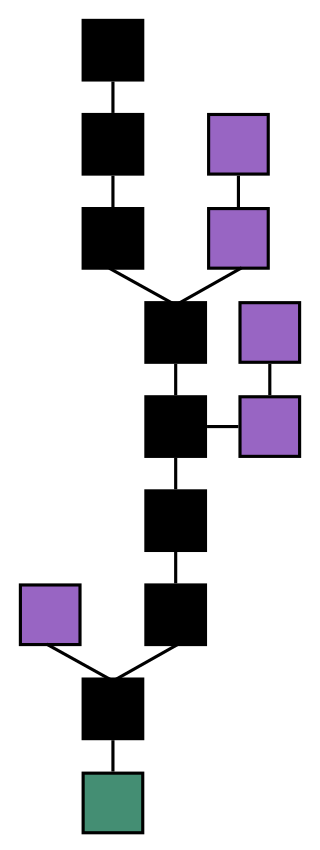
\includegraphics[scale=0.3, angle=270]{myfigs/wikipedia-Blockchain.jpg}
		\caption{An example of a blockchain}
	\end{figure}
\end{enumerate}
\end{frame}
\begin{frame}\frametitle{Background II} 
\begin{enumerate}
	\item[] - \textcolor{orange}{Smart Contract}: \sout{A smart contract is a computer protocol intended to digitally facilitate, verify, or enforce the negotiation or performance of a contract.} \textcolor{red}{TL;DR -- Code is Law; Algorithmic Governance.}
	\item[$\bullet$] Secure Multiparty Computation (MPC or SMC)
	\item[] - Secure multi-party computation is a subfield of cryptography with the goal of creating methods for parties to \uwave{\textcolor{orange}{jointly}} compute a function over their inputs while \dashuline{keeping those inputs private}. 
\end{enumerate}
\end{frame}


\begin{frame}\frametitle{An Example of MPC: Average Salary Problem} 
\textcolor{orange}{\textbf{Problem Description}}: An employee wishes to know whether his/her salary exceeds the average level of that in the company. Of course, he/she needs to do it in a privacy-preserving manner: after the protocol, \textcolor{red}{only} the number of \uuline{average salary} should be calculated. How to do this?

\vspace{0.5cm}

\textcolor{blue}{\textbf{Solution}}: Adding a random number and then 
\end{frame}

\begin{frame}\frametitle{An Example of MPC: Average Salary Problem II}
\begin{figure}
	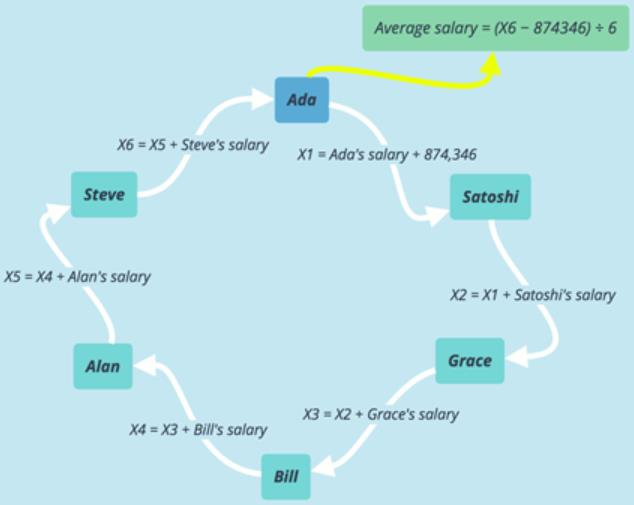
\includegraphics[width=3.2 in, height=2.5in]{myfigs/averagesalary.jpg}
\end{figure}
\colorbox{blue}{Remark}: This protocol will become meaningless in two-party setting. 
\end{frame}

\begin{frame}\frametitle{An Example of MPC: Yao's Millionaires' Problem} 
\textcolor{orange}{\textbf{Problem Description}}: Two millionaires, Alice and Bob, who are interested in knowing whom of them is richer \dotuline{without revealing their actual wealth}.
\begin{figure}
	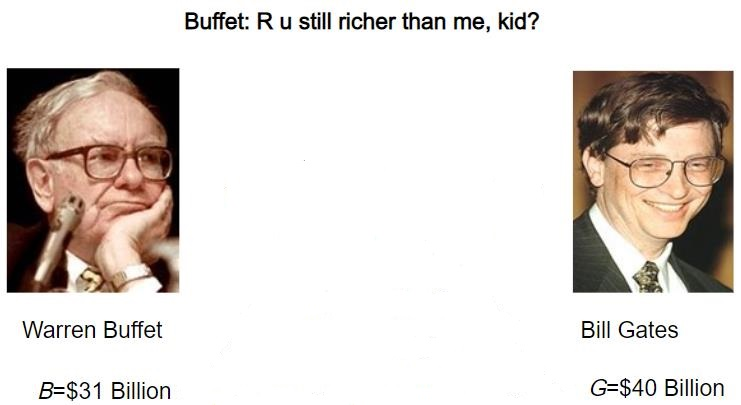
\includegraphics[width=3.1 in, height=1.9 in]{myfigs/SMC.jpg}
\end{figure}
\pause
\colorbox{blue}{A joke}: It's not an example for Yao's Millionaires' Problem and it is exactly an example for Yao's \uwave{\textcolor{orange}{\textbf{B(M)illionaires}}}' Problem...

\end{frame}


\begin{frame}\frametitle{A Solution to Yao's Millionaires' Problem (without explanation)} 

\end{frame}


\begin{frame}\frametitle{Limitation of MPC: Marriage Proposal Problem} 
\textcolor{orange}{\textbf{Problem Description}}: Alice and Bob are in an ambiguous state. Both of them would very very like to know if the other party wishes to marry her/him, and as usual, in a ``private'' manner.
\end{frame}


\begin{frame}\frametitle{Limitation of MPC: Marriage Proposal Problem} 
\begin{figure}
	
\includegraphics[width=0.8\textwidth, height=0.3\textheight]{myfigs/gaomu1.jpg}
\end{figure}
\pause
\begin{figure}
	
\includegraphics[width=0.8\textwidth, height=0.3\textheight]{myfigs/gaomu2.jpg}
\end{figure}
\end{frame}

\begin{frame}\frametitle{Limitation of MPC: Marriage Proposal Problem} 

\end{frame}


\begin{frame}\frametitle{Motivation} 
\begin{center}
\fbox{\begin{minipage}{0.9\textwidth}
\flushleft
\Large
- Online gambling \newline \vspace{1.5cm}

- Online lottery \newline \vspace{1.5cm}

- Other activities involving mutual trust and \uuline{\textcolor{yellow}{money}}
\end{minipage}
}
\end{center}


\end{frame}

%%%%%%%%%%%%%%%%%%%%%%%%%%%%%%%%%%%%%%%%%%%%%%%%%%

\section{Preliminaries}

\begin{frame}\frametitle{Definition of MPC} 

\end{frame}


\begin{frame}\frametitle{(Cryptographic) Signature Schemes} 
A \textcolor{orange}{\textbf{digital signature}} is a mathematical scheme for verifying the authenticity of digital messages or documents. A valid digital signature, where the prerequisites are satisfied, gives a recipient very strong reason to believe that the message was created by a known sender (\textcolor{blue}{\underline{authentication}}), and that the message was not altered in transit (\textcolor{blue}{\underline{integrity}}).
\begin{figure}
	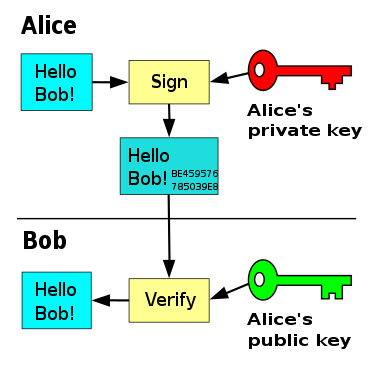
\includegraphics[width=2.6 in, height=1.9in]{myfigs/wikipedia-signature.jpg}
	\caption{The MultiPlayersLottery protocol}
\end{figure}
\end{frame}



\begin{frame}\frametitle{(Cryptographic) Hash Functions I}
A \textcolor{orange}{\textbf{cryptographic hash function}} is a mathematical algorithm that maps data of arbitrary size to a bit string of a fixed size ($\{0,1\}^{\textcolor{red}{*}} \rightarrow \{0,1\}^{\textcolor{yellow}{n}}$, just like \textcolor{blue}{compression}) and is a \textcolor{blue}{one-way} function, that is, a function which is practically infeasible to invert. Besides, \textcolor{blue}{collision-resistance}, \textcolor{blue}{pseudo-randomness} and \textcolor{blue}{avalanche effect} are also required. Let's explain them in an \textit{informal} way.
\begin{enumerate}
	\item compression: This is natural otherwise why we need hash?
	\item one-wayness: Mainly for security purpose.
	\item collision-resistance: The most import point for cryptographic hash.
	\item pseudomness: Looks like ``real random''.
	\item avalanche effect: Also for security reason.
\end{enumerate}
\end{frame}
\begin{frame}\frametitle{(Cryptographic) Hash Functions II}
\begin{figure}
	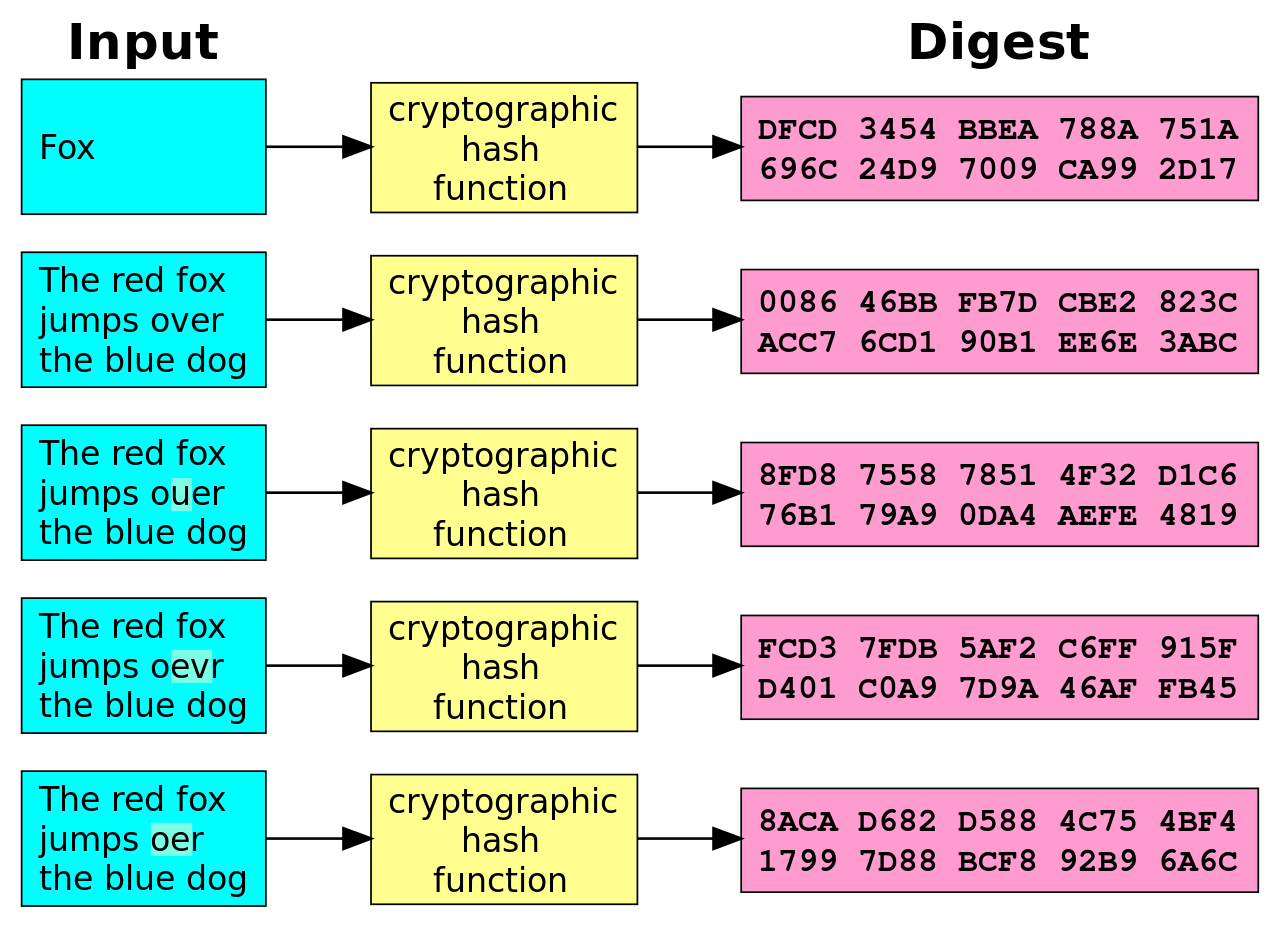
\includegraphics[width=3.8 in, height=2.2in]{myfigs/wikipedia-CryptographicHashFunction.jpg}
	\caption{Avalanche effect of cryptographic hash function}
\end{figure}
\end{frame}



\begin{frame}\frametitle{Commitment Schemes} 
A \textcolor{orange}{\textbf{commitment scheme}} is a cryptographic primitive that allows one to commit to a chosen value (or chosen statement) while keeping it hidden to others, with the ability to reveal the committed value later. Commitment schemes are designed so that a party cannot change the value or statement after they have committed to it: that is, commitment schemes are binding.
\begin{figure}
	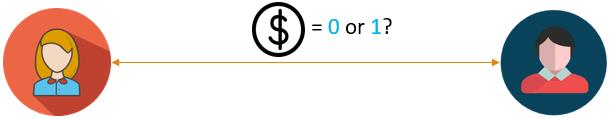
\includegraphics[width=3.6 in, height=0.7in]{myfigs/coin-flipping.jpg}
	\caption{Example: coin flipping on the internet}
\end{figure}
\end{frame}

\begin{frame}\frametitle{Bitcoin Crash Course: Procedure of Spending a Bitcoin} 
\begin{alertblock}{Pivotal points behind a transaction:}
Alice drafts a transaction alerting that she transfers \colorbox{blue}{$v$} money/coin to Bob. And other users accept this behavior.
\end{alertblock}
\begin{block}{Let's dive deeper into this:}
1. Alice references an (or multiple) existing transaction(s) in which she is the receiver of a certain amount of money. The number of money should be at least equal to \colorbox{blue}{$v$}. \newline\textcolor{red}{$\Longrightarrow$ //There exists some \underline{unspent} money.}

2. Alice signs the transaction with her private key. \newline\textcolor{red}{$\Longrightarrow$ //Alice: I am indeed the owner of the money because I can use it.}

3. Alice write in the transaction that she transfers the money to the public key of Bob. \newline\textcolor{red}{$\Longrightarrow$ //Alice: The receiver of my money is Bob, he can use it after this transaction.}
\end{block}

\end{frame}

\begin{frame}\frametitle{Bitcoin Crash Course: Generalizing Signature to Script} 

\end{frame}

\begin{frame}\frametitle{Properties of Bitcoin} 

\end{frame}


%%%%%%%%%%%%%%%%%%%%%%%%%%%%%%%%%%%%%%%%%%%%%%%%%%

\section{Main Protocols}

\begin{frame}\frametitle{Timed Commitment} 
\begin{figure}
	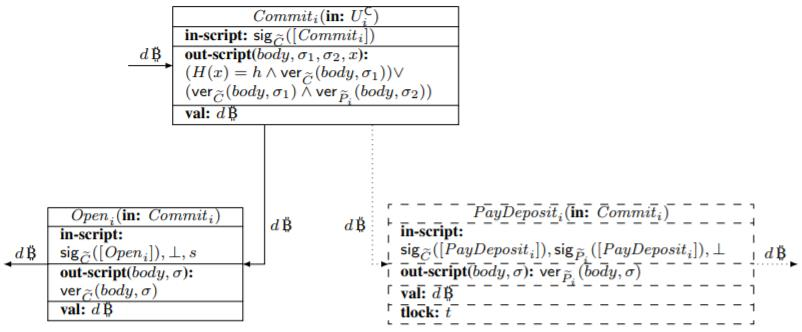
\includegraphics[width=4.6 in]{myfigs/timed-commitment.jpg}
	\caption{The timed-commitment scheme}
\end{figure}
\end{frame}


\begin{frame}\frametitle{A Test Trial: The Put Money Transaction}
\begin{figure}
	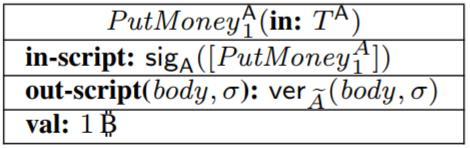
\includegraphics[width=2.2 in]{myfigs/PutMoney1.jpg}
\end{figure}
\end{frame}

\begin{frame}\frametitle{Put Money}
\begin{figure}
	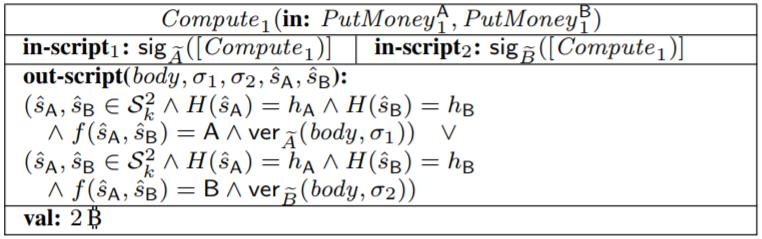
\includegraphics[width=3 in, height=1.2 in]{myfigs/Compute1.jpg}
\end{figure}

\end{frame}
\begin{frame}\frametitle{Put Money}
\begin{figure}
	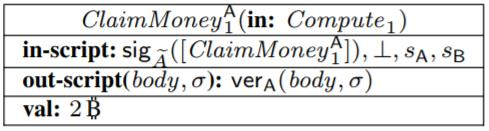
\includegraphics[width=2 in]{myfigs/ClaimMoney1.jpg}
\end{figure}

\end{frame}


\begin{frame}\frametitle{Timed Commitment} 

\end{frame}



\begin{frame}\frametitle{The Whole Procedure of Multi-Player Lottery Protocol} 
\begin{figure}
	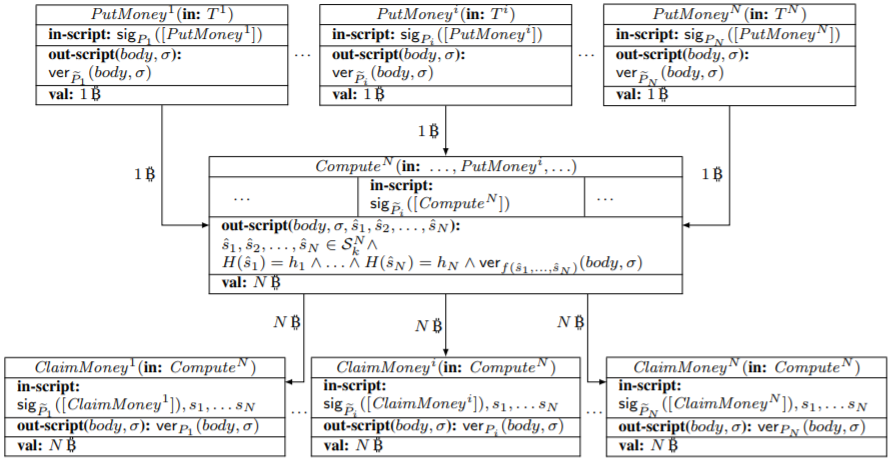
\includegraphics[width=4.6 in]{myfigs/lotteryprotocol1.jpg}
	\caption{The MultiPlayersLottery protocol}
\end{figure}
\end{frame}

%%%%%%%%%%%%%%%%%%%%%%%%%%%%%%%%%%%%%%%%%%%%%%%%%%

\section[conclu]{Conclusion}


\begin{frame}\frametitle{}
\Huge
\begin{center}
\rotatebox{15}{Thanks! Any Questions?}
\end{center}
\end{frame}

%%%%%%%%%%%%%%%%%%%%%%%%%%%%%%%%%%%%%%%%%%%%%%%%%%
% The contents in these frames are added by myself.
%% The end.
%%%%%%%%%%%%%%%%%%%%%%%%%%%%%%%%%%%%%%%%%%%%%%%%%%



%%%%%%%%%%%%%%%%%%%%%%%%%%%%%%%%%%%%%%%%%%%%%%%%%%
%%%%%%%%%%%%%%%%%%%%%%%%%%%%%%%%%%%%%%%%%%%%%%%%%%
%%%%%%%%%%%%%%%%%%%%%%%%%%%%%%%%%%%%%%%%%%%%%%%%%%
%%%%%%%%%%%%%%%%%%%%%%%%%%%%%%%%%%%%%%%%%%%%%%%%%%
%%%%%%%%%%%%%%%%%%%%%%%%%%%%%%%%%%%%%%%%%%%%%%%%%%
%%%%%%%%%%%%%%%%%%%%%%%%%%%%%%%%%%%%%%%%%%%%%%%%%%
%%%%%%%%%%%%%%%%%%%%%%%%%%%%%%%%%%%%%%%%%%%%%%%%%%
%%%%%%%%%%%%%%%%%%%%%%%%%%%%%%%%%%%%%%%%%%%%%%%%%%
%%%%%%%%%%%%%%%%%%%%%%%%%%%%%%%%%%%%%%%%%%%%%%%%%%
%%%%%%%%%%%%%%%%%%%%%%%%%%%%%%%%%%%%%%%%%%%%%%%%%%
%%%%%%%%%%%%%%%%%%%%%%%%%%%%%%%%%%%%%%%%%%%%%%%%%%
%%%%%%%%%%%%%%%%%%%%%%%%%%%%%%%%%%%%%%%%%%%%%%%%%%
%%%%%%%%%%%%%%%%%%%%%%%%%%%%%%%%%%%%%%%%%%%%%%%%%%
%%%%%%%%%%%%%%%%%%%%%%%%%%%%%%%%%%%%%%%%%%%%%%%%%%
%%%%%%%%%%%%%%%%%%%%%%%%%%%%%%%%%%%%%%%%%%%%%%%%%%
%%%%%%%%%%%%%%%%%%%%%%%%%%%%%%%%%%%%%%%%%%%%%%%%%%
%%%%%%%%%%%%%%%%%%%%%%%%%%%%%%%%%%%%%%%%%%%%%%%%%%
%%%%%%%%%%%%%%%%%%%%%%%%%%%%%%%%%%%%%%%%%%%%%%%%%%
%%%%%%%%%%%%%%%%%%%%%%%%%%%%%%%%%%%%%%%%%%%%%%%%%%
%%%%%%%%%%%%%%%%%%%%%%%%%%%%%%%%%%%%%%%%%%%%%%%%%%
%%%%%%%%%%%%%%%%%%%%%%%%%%%%%%%%%%%%%%%%%%%%%%%%%%
%%%%%%%%%%%%%%%%%%%%%%%%%%%%%%%%%%%%%%%%%%%%%%%%%%
%%%%%%%%%%%%%%%%%%%%%%%%%%%%%%%%%%%%%%%%%%%%%%%%%%
%%%%%%%%%%%%%%%%%%%%%%%%%%%%%%%%%%%%%%%%%%%%%%%%%%



%%%%%%%%%%%%%%%%%%%%%%%%%%%%%%%%%%%%%%%%%%%%%%%%%%
% comment out all the contents of the former file
\iffalse
%%%%%%%%%%%%%%%%%%%%%%%%%%%%%%%%%%%%%%%%%%%%%%%%%%

%--------------------------------------------------------------------------------
%	PRESENTATION SLIDES

%------------------------------------------------
\section{Precessão} 


\begin{frame}
\frametitle{O que é precessão?}
\begin{itemize}
\item Precessão é a rotação do eixo de rotação de um objeto em torno de um segundo eixo.
\item É criado pelo torque da força peso (em geral) sobre o centro de massa quando o objeto está já em rotação. 
\pause
\item Não é um fenômeno intuitivo.
\item Porém mostra o quão sensacional é a grandeza momento angular!
\end{itemize}
\end{frame}



\begin{frame}
\frametitle{Precessão da Terra}
\begin{itemize}
\item O eixo de rotação da Terra sofre precessão: ele rotaciona em torno de outro eixo com um período de 26 mil anos.
\item O torque causador é exercido pela atração gravitacional da Lua e Sol.
\pause
\item Ainda há o movimento de nutação: oscilação em torno do cone de precessão.
\item Nutação e precessão da Terra são devido ao torque exercido pela Lua, Sol e outros planetas e pelo fato da Terra não ser uma esfera.
\end{itemize}
\end{frame}

\begin{frame}
\frametitle{Precessão da Terra}
\begin{figure}
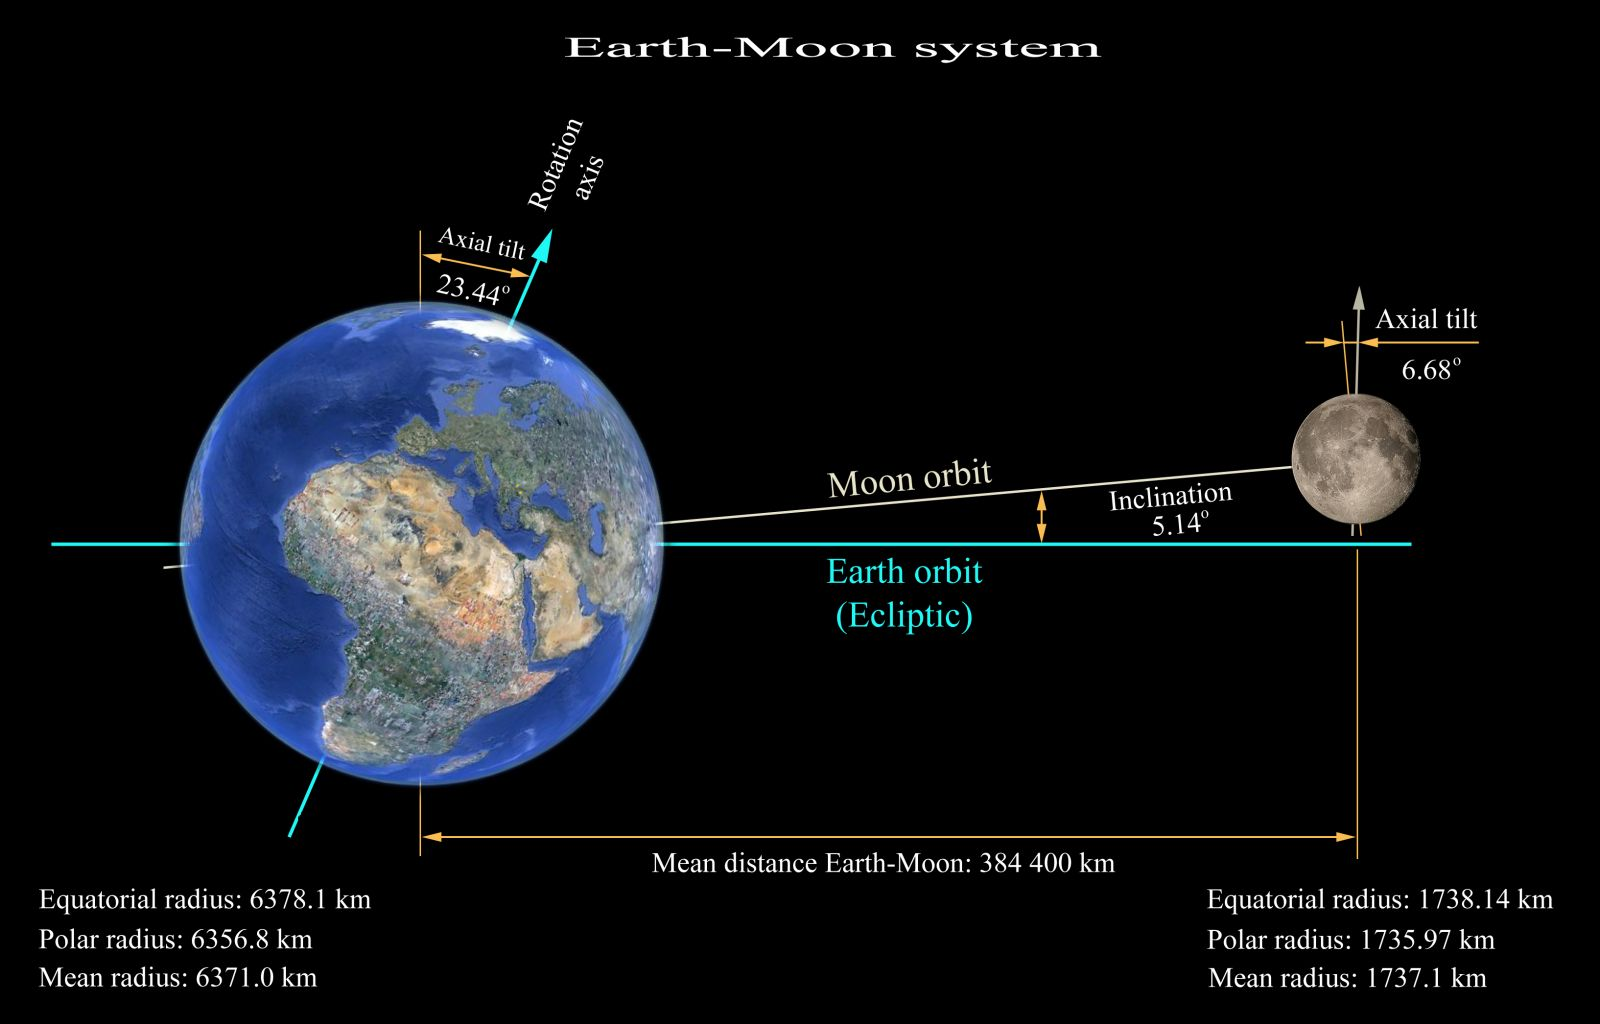
\includegraphics[width=4.0 in]{figuras/earth_moon_system.jpg}
%\caption{Fonte: \cite{Serway2014}.}
\end{figure}
\end{frame}


\begin{frame}
\frametitle{Precessão da Terra}
\begin{figure}
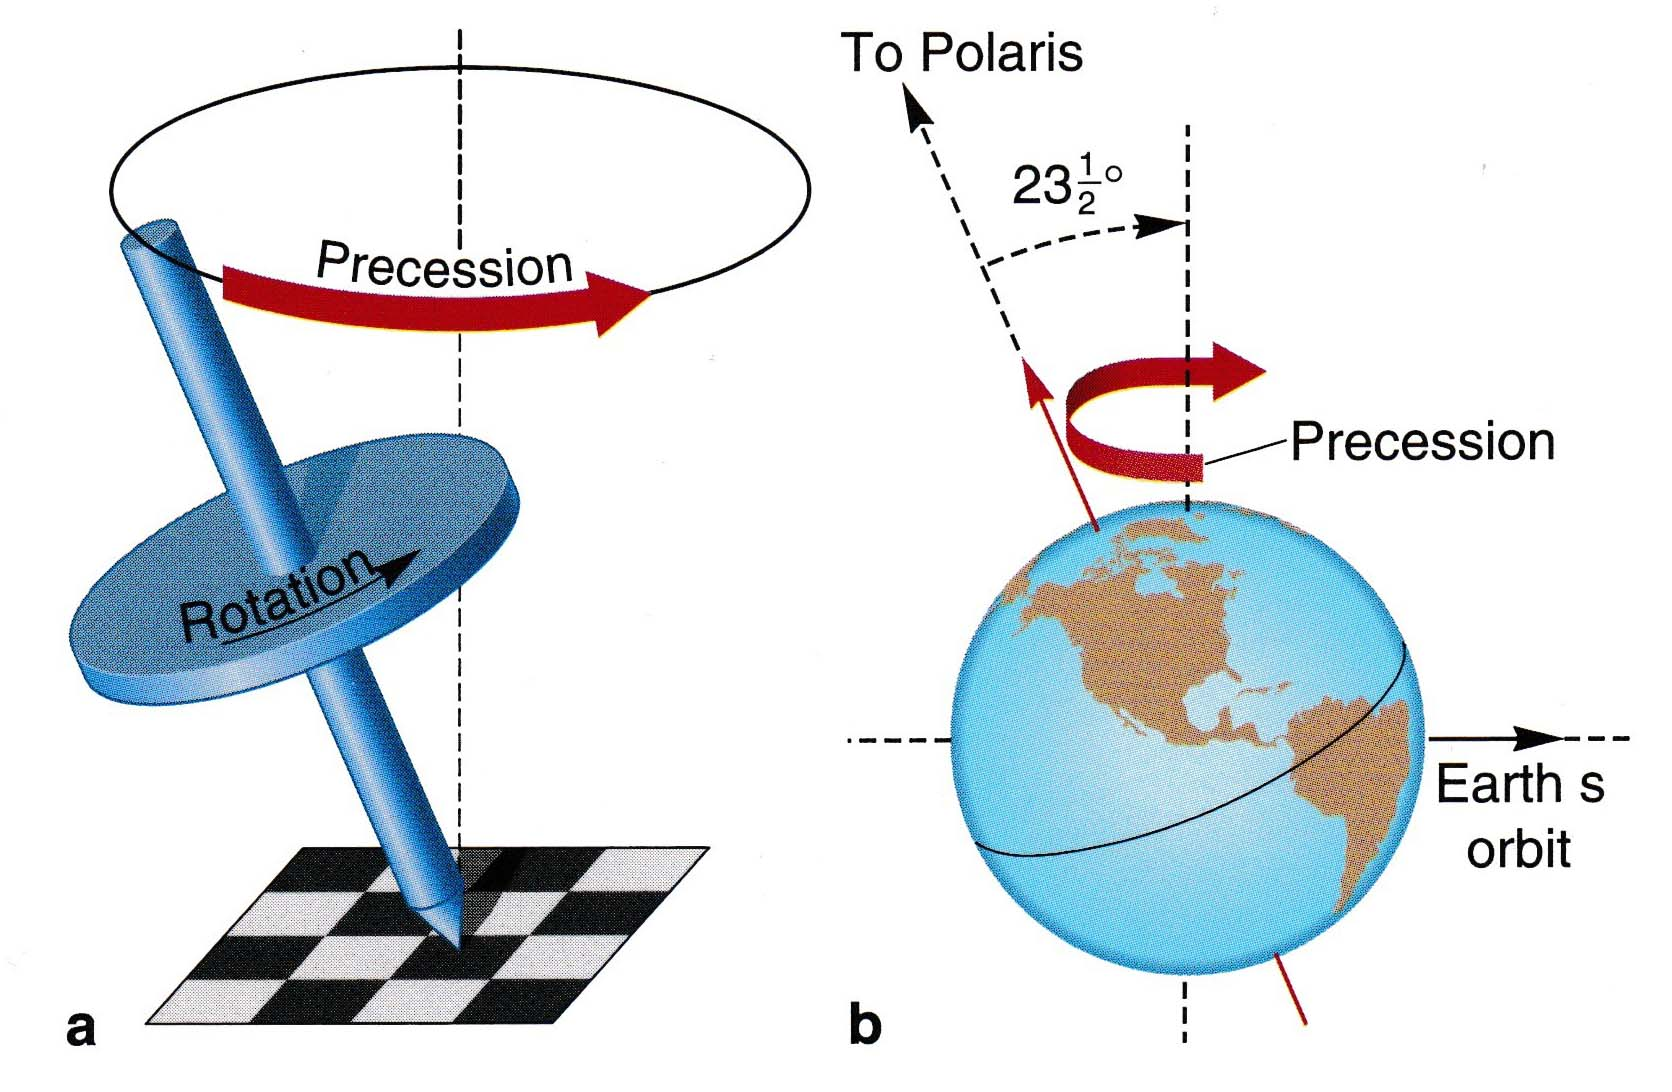
\includegraphics[width=3.9 in]{figuras/precession1a.jpg}
%\caption{Fonte: \cite{Serway2014}.}
\end{figure}
\end{frame}

\begin{frame}
\frametitle{Precessão da Terra}
\begin{figure}
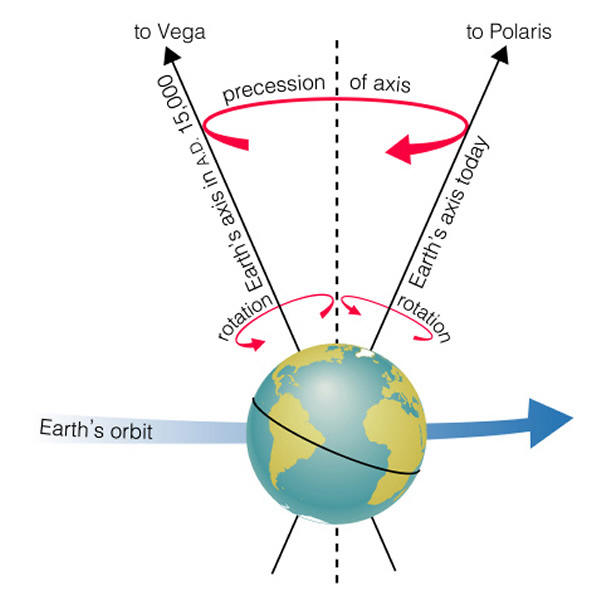
\includegraphics[width=2.2 in]{figuras/earthprecess.jpg}
%\caption{Fonte: \cite{Serway2014}.}
\end{figure}
\end{frame}






\begin{frame}
\frametitle{Precessão da Terra}
\begin{figure}
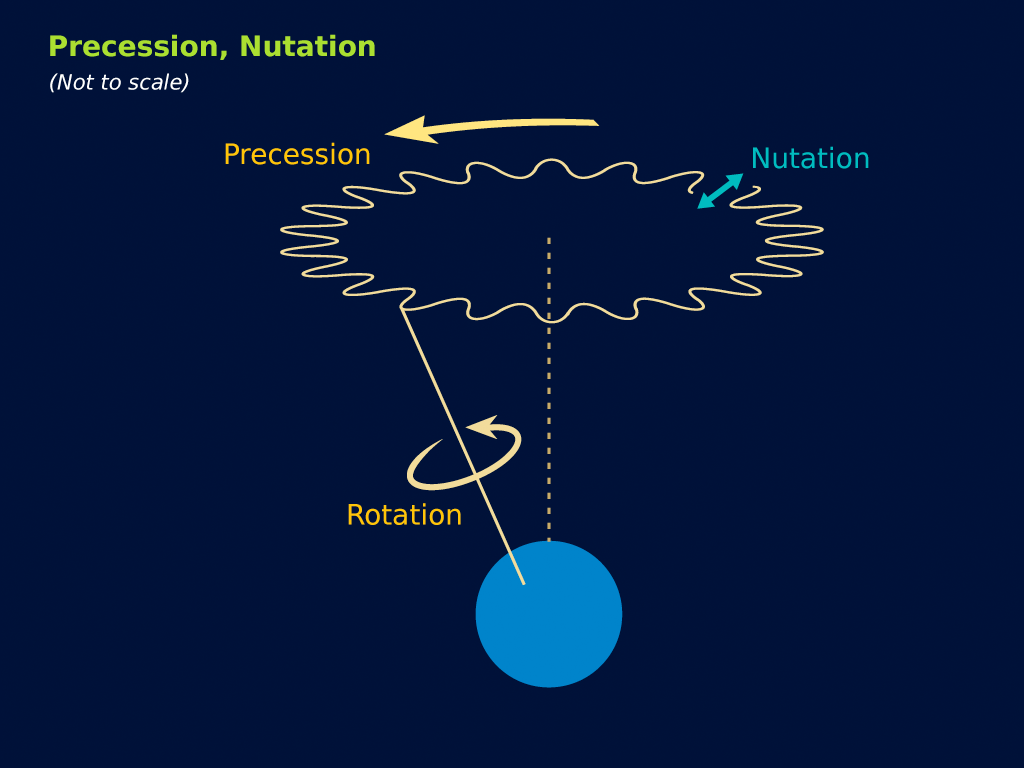
\includegraphics[width=3.7 in]{figuras/Precession_Nutation.png}
%\caption{Fonte: \cite{Serway2014}.}
\end{figure}
\end{frame}


\section{Giroscópio}


\begin{frame}
\frametitle{O que é giroscópio?}
\begin{itemize}
\item Giroscópio é um dispositivo contendo um rotor que rotaciona e outra parte externa que a sustenta. 
\item Independente de como a parte externa é suspensa a parte interna pode rotacionar livremente.
\item O atrito do suporte pode impedir uma rotação continuada do rotor.
\item Uma das aplicações do giroscópio é a observação da precessão.
\item Dentre as várias aplicações, o giroscópio é utilizado também para se observar a precessão.
\end{itemize}
\end{frame}


\begin{frame}
\begin{figure}
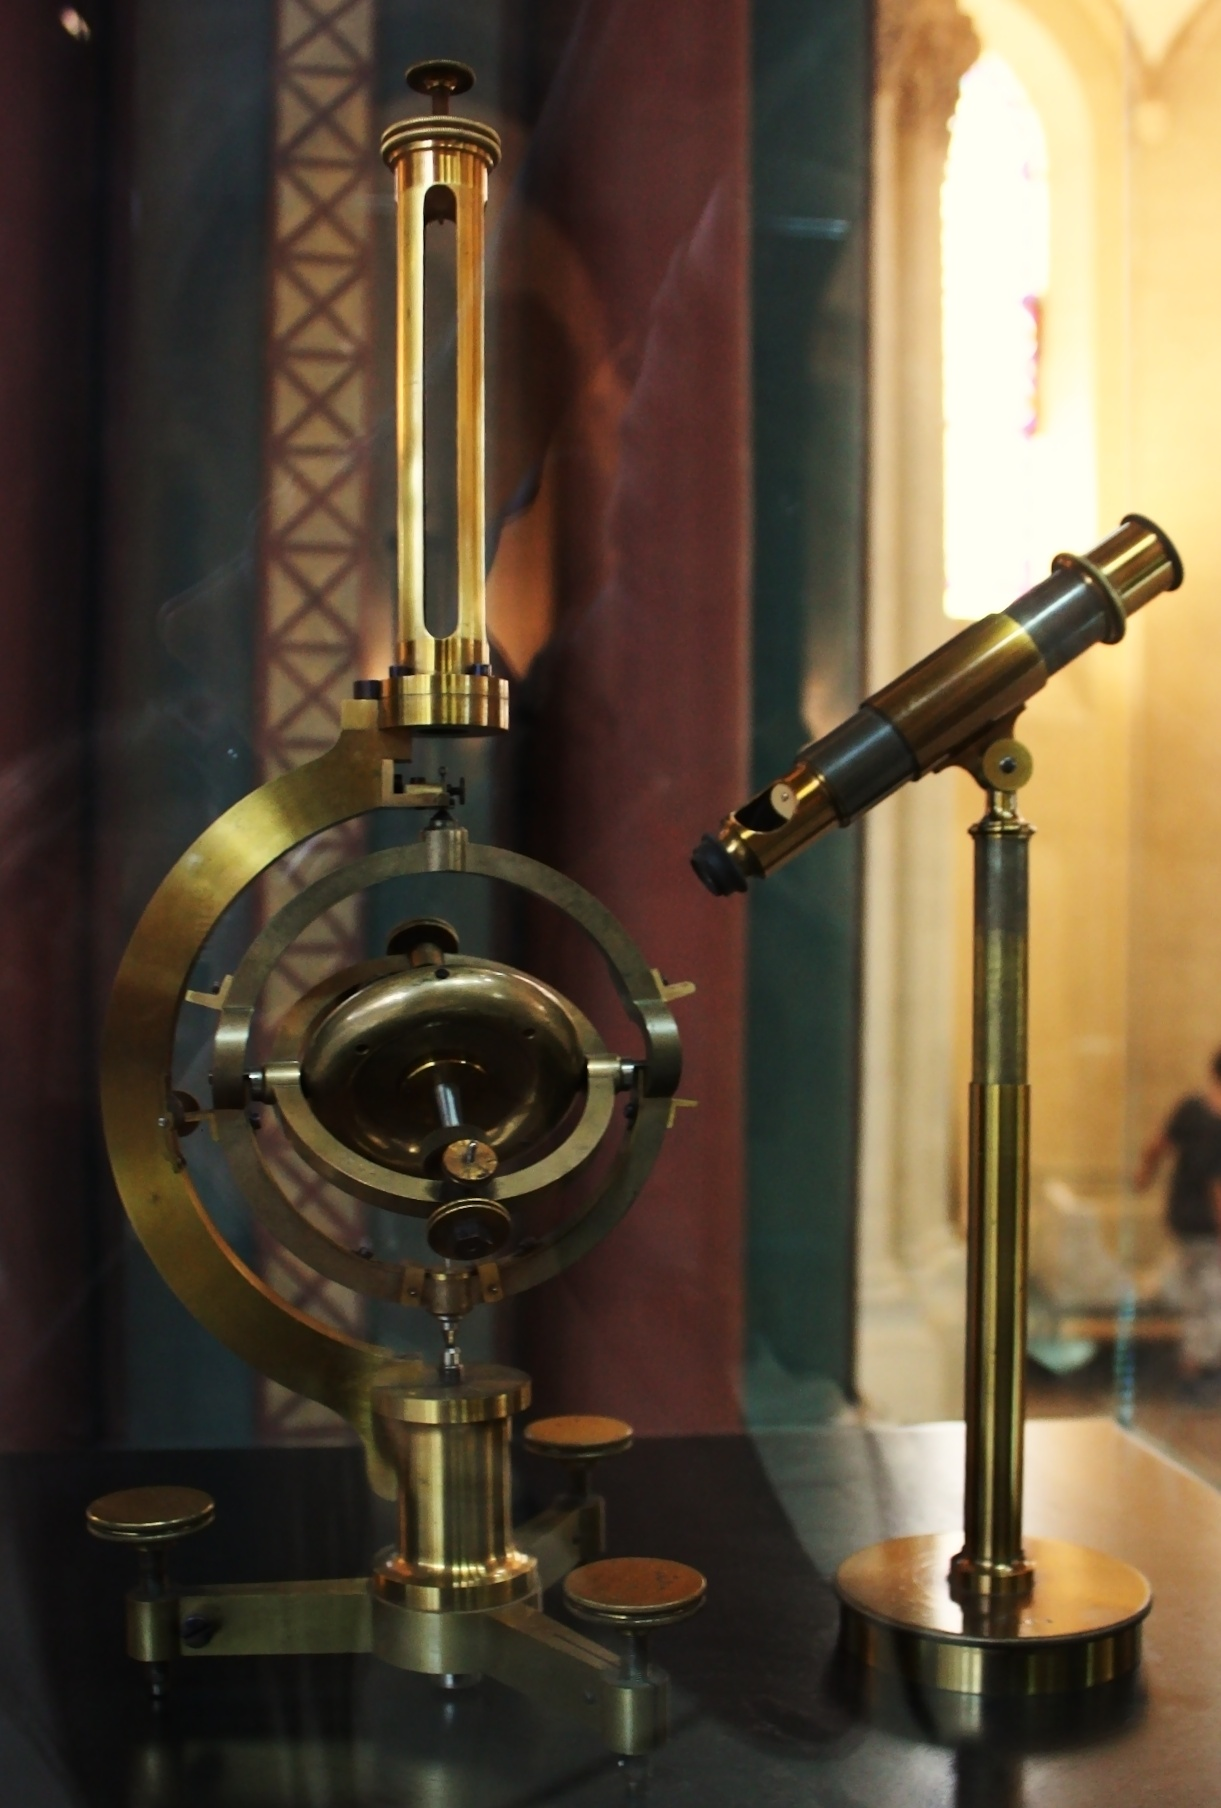
\includegraphics[width=2.0 in]{figuras/giroscopio_foucault.jpg}
\end{figure}
Giroscópio feito em 1852 por Léon Foucault.
\end{frame}

\begin{frame}
\begin{figure}
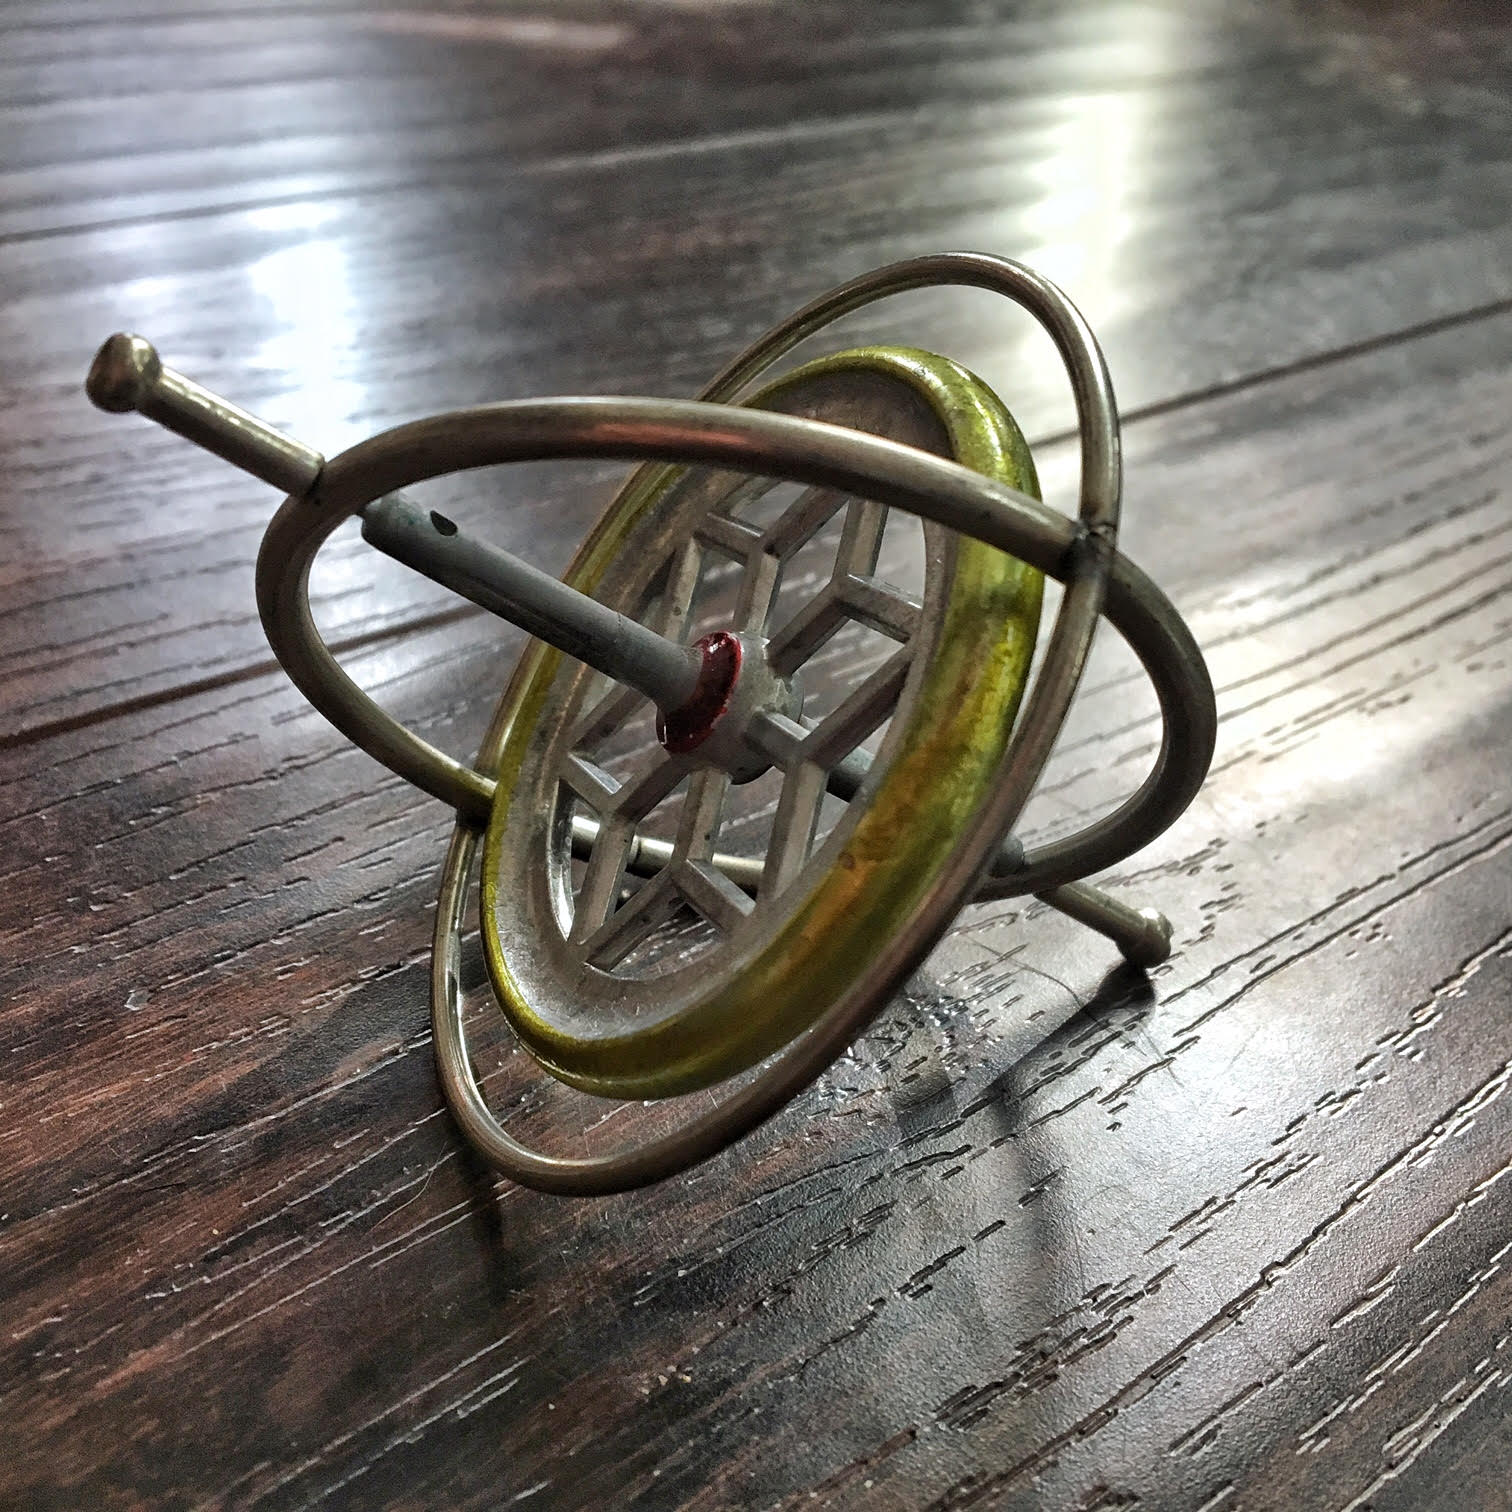
\includegraphics[width=3.0 in]{figuras/Gyroscope.jpg}
\end{figure}
Giroscópio de brinquedo da TEDCO Toys: criado em 1917.
\end{frame}

\begin{frame}
\begin{figure}
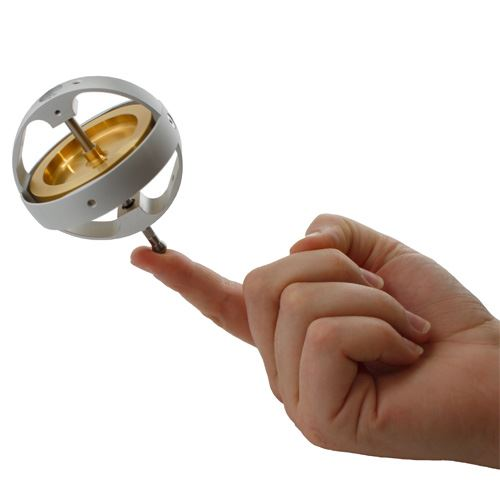
\includegraphics[width=3.0 in]{figuras/gyro3.jpg}
\end{figure}
\end{frame}

\begin{frame}
\begin{figure}
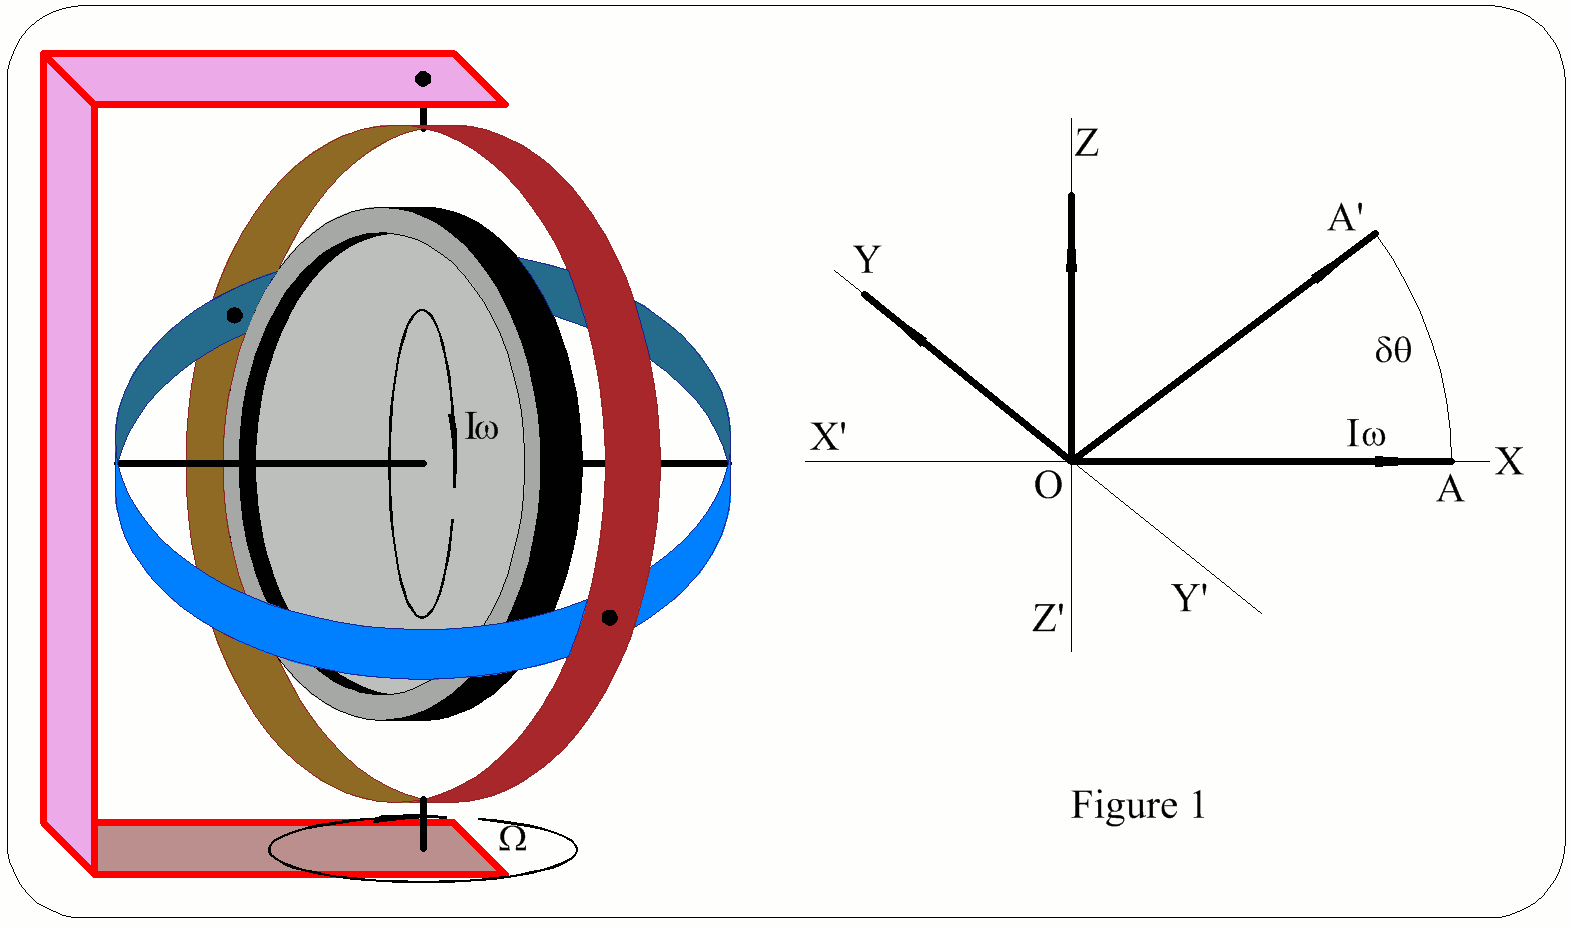
\includegraphics[width=4.2 in]{figuras/G1a.png}
\end{figure}
\end{frame}

\begin{frame}
\begin{figure}
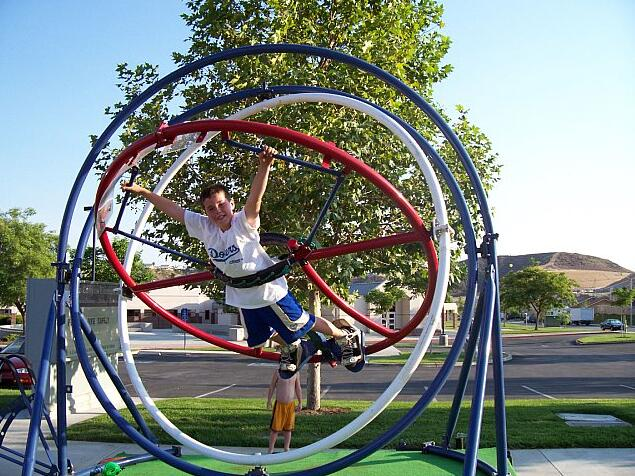
\includegraphics[width=3.9 in]{figuras/Human-Gyroscope.jpg}
\end{figure}
\end{frame}



\section{Modelo Teórico}

\begin{frame}
\frametitle{Definições}
%\framesubtitle{Definições}
\begin{itemize}
\item Grandezas vetoriais em negrito: {\color{red}$a=$} escalar e {\color{red}$\textbf{a}=$} vetor.
\item Momento Angular: {\color{red}$\textbf{L} = \textbf{r} \times \textbf{p} = m\textbf{r} \times \textbf{v} $}.
\item Torque: {\color{red}$\bm{\tau} = \textbf{r} \times \textbf{F}$}.
\item Torque da força peso: {\color{red}$\bm{\tau}_p = m\textbf{r} \times \textbf{g}$}.
\item Lei de Newton angular: {\color{red}$\bm{\tau} = \dfrac{d\textbf{L}}{dt}$}.
\end{itemize}
\end{frame}

\begin{frame}
%\frametitle{Introdu\c{c}\~ao}
\begin{figure}
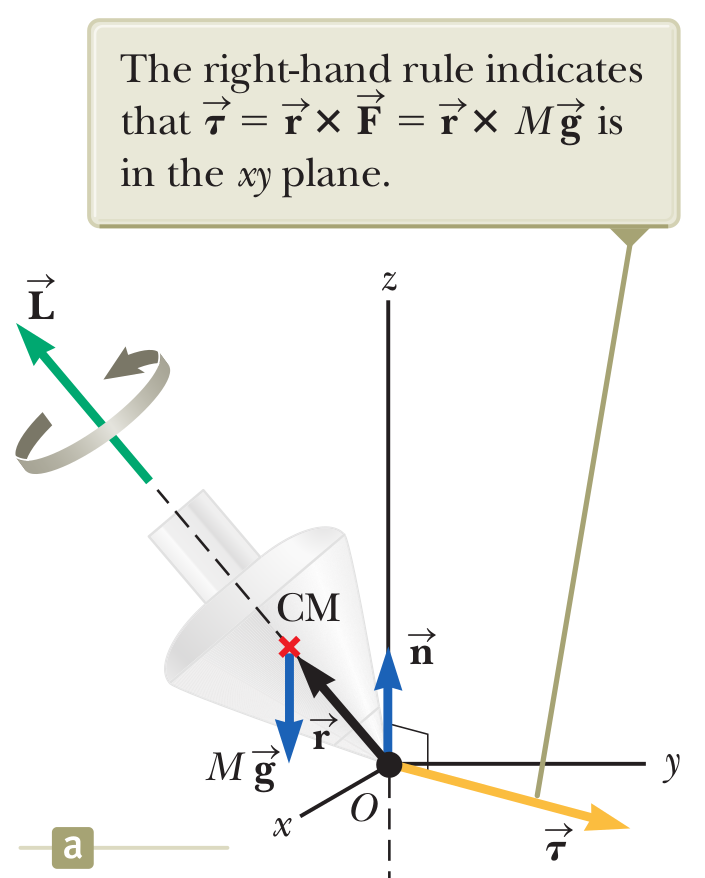
\includegraphics[width=2.2 in]{figuras/peao1.png}
\pause
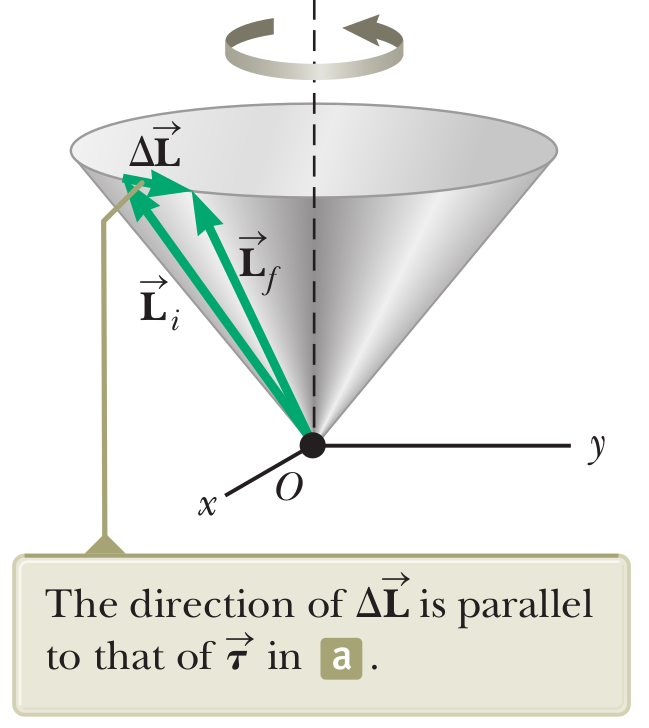
\includegraphics[width=2.2 in]{figuras/peao2.png}
\caption{Fonte: \cite{Serway2014}.}
\end{figure}
\end{frame}



\begin{frame}
\frametitle{Definições}
\begin{itemize}
\item O peão sofre duas forças: peso atuando no centro de massa e normal do chão no ponto de contato com o chão.
\item Seja {\color{red}$\textbf{r}$} no plano $yz$.
\item O peso faz um torque {\color{red}$\bm{\tau} = M\textbf{r} \times \textbf{g}=\hat{\textbf{i}}\tau$} paralelo ao eixo $x$.
\pause
\item Logo, da Lei de Newton: {\color{red}$d\textbf{L} = \bm{\tau}dt$}.
\item Isso faz o momento angular girar: {\color{red}$\textbf{L} = \textbf{L}_0 + \bm{\tau}dt$}.
\item Já que {\color{red}$\textbf{L}_0 \cdot \bm{\tau}=0$}: {\color{red}$\textbf{L}_0$} e {\color{red}$\bm{\tau}$} são perpendiculares.
\pause
\item Assim apenas a direção do momento angular {\color{red}$\textbf{L}$} é alterada.
\item O movimento de {\color{red}$\textbf{L}$} é chamado de precessão.
\end{itemize}
\end{frame}


\begin{frame}
%\frametitle{Introdu\c{c}\~ao}
\begin{figure}
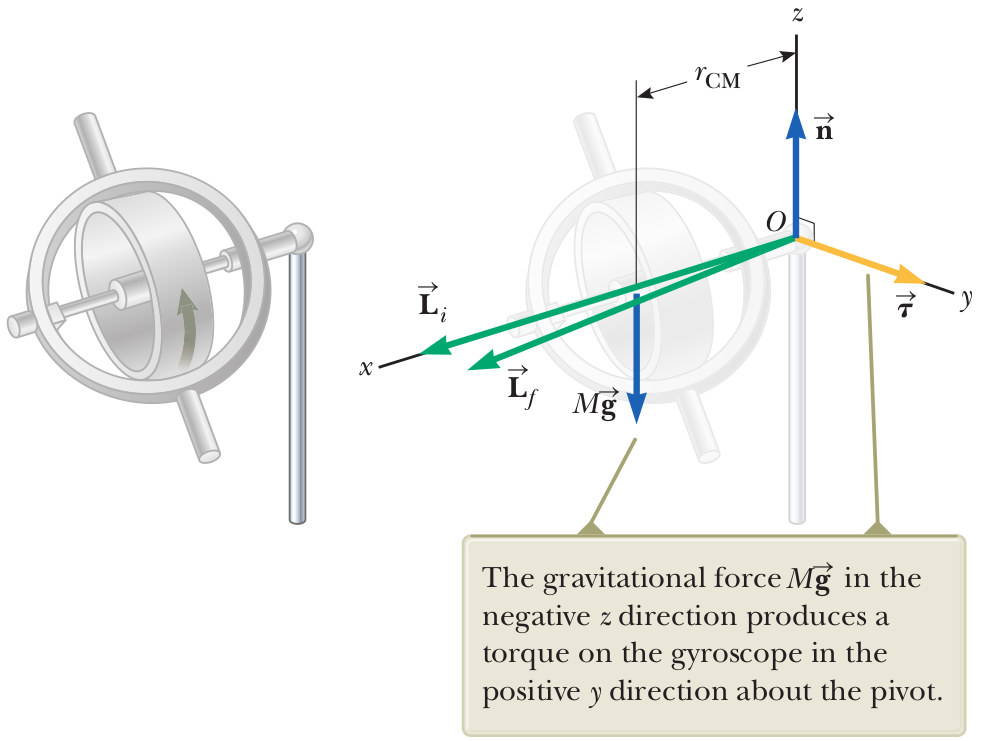
\includegraphics[width=3.6 in]{figuras/giroscopio1.png}
\caption{Fonte: \cite{Serway2014}.}
\end{figure}
\end{frame}


\begin{frame}
%\frametitle{Introdu\c{c}\~ao}
\begin{figure}
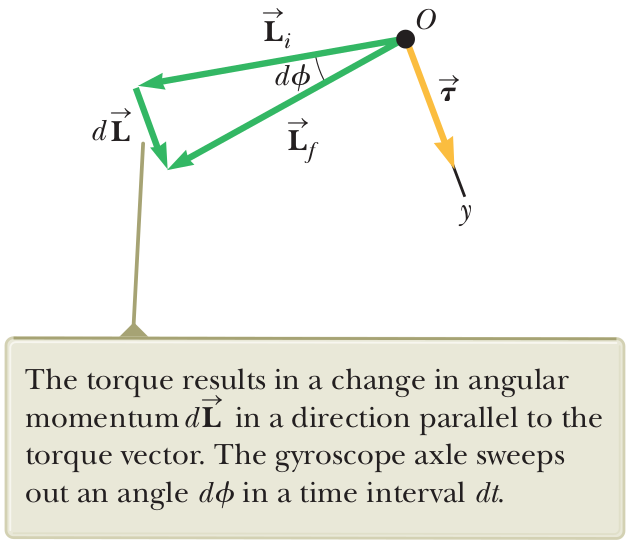
\includegraphics[width=3.4 in]{figuras/giroscopio2.png}
\caption{Fonte: \cite{Serway2014}.}
\end{figure}
\end{frame}


\begin{frame}
\frametitle{Velocidade angular de precessão}
\begin{itemize}
\item Do triângulo da figura anterior: {\color{red}$d\phi = \dfrac{dL}{L} = \dfrac{\tau dt}{L} = \dfrac{r F  }{I \omega}dt$}.
\item Logo a velocidade angular de precessão é:
{\color{red}\begin{equation}
\Omega = \dfrac{d\phi}{dt} = \dfrac{F r}{I \omega}, \nonumber
\end{equation}}
onde {\color{red}$F$} é a força que executa o torque.
\item Em geral é o peso {\color{red}$F=Mg$}.
\item Este resultado é valido quando {\color{red}$\Omega << \omega$}.
\end{itemize}
\end{frame}

%---------------------------------------------------



%-------------------------------------------------------
\section{Aplicações}
%-------------------------------------------------------


\begin{frame}
\frametitle{Aplicações}
\begin{itemize}
\item Giroscópios são dispositivos que mantem uma rotação independente da maneira com que são suportados.
\item Que aplicação isso teria?
\pause
\item Suponha que o giroscópio tenha seu rotor rotacionando. Quando o suporte é rotacionado, há então um movimento relativo entre ambos.
\item As aplicações residem ai: detecção desse movimento relativo!
\item Conectando o giroscópio em algo, pode-se saber quando esse algo rotaciona e então executar alguma função.
\end{itemize}
\end{frame}


\begin{frame}
\frametitle{Aplicações}
\begin{itemize}
\item Conectando o giroscópio em alguma estrutura, pode-se saber quando esse algo rotaciona e então executar alguma função.
\item Pode-se então determinar o ângulo de rotação (posição angular) dessa estrutura.
\item Isso significa então que podemos orientar essa estrutura da forma desejada.
\pause
\item A maior aplicação de giroscópios é estabilização!
\end{itemize}
\end{frame}

\begin{frame}
\frametitle{Estabilização}
\begin{itemize}
\item Câmeras, aeronaves e veículos podem ser mais estáveis com um sistema ativo que, dado a rotação do giroscópio, executa o movimento contrário para o veículo permanecer imóvel. 
\item Os instrumentos no helicóptero que indicam sua orientação são baseados em giroscópios.
\end{itemize}
\end{frame}

\begin{frame}
\frametitle{Smartphones e tablets}
\begin{itemize}
\item Giroscópios "eletrônicos" (MEMS-based) são amplamente utilizados em celulares e tables.
\item Combinado com acelerômetro e magnetômetro, obtém-se resultados precisos para a localização, posição e movimento do aparelho.
\item Aplicativos diversos exploram essa capacidade.
\end{itemize}
\end{frame}




\begin{frame}
%\frametitle{Introdu\c{c}\~ao}
\begin{figure}
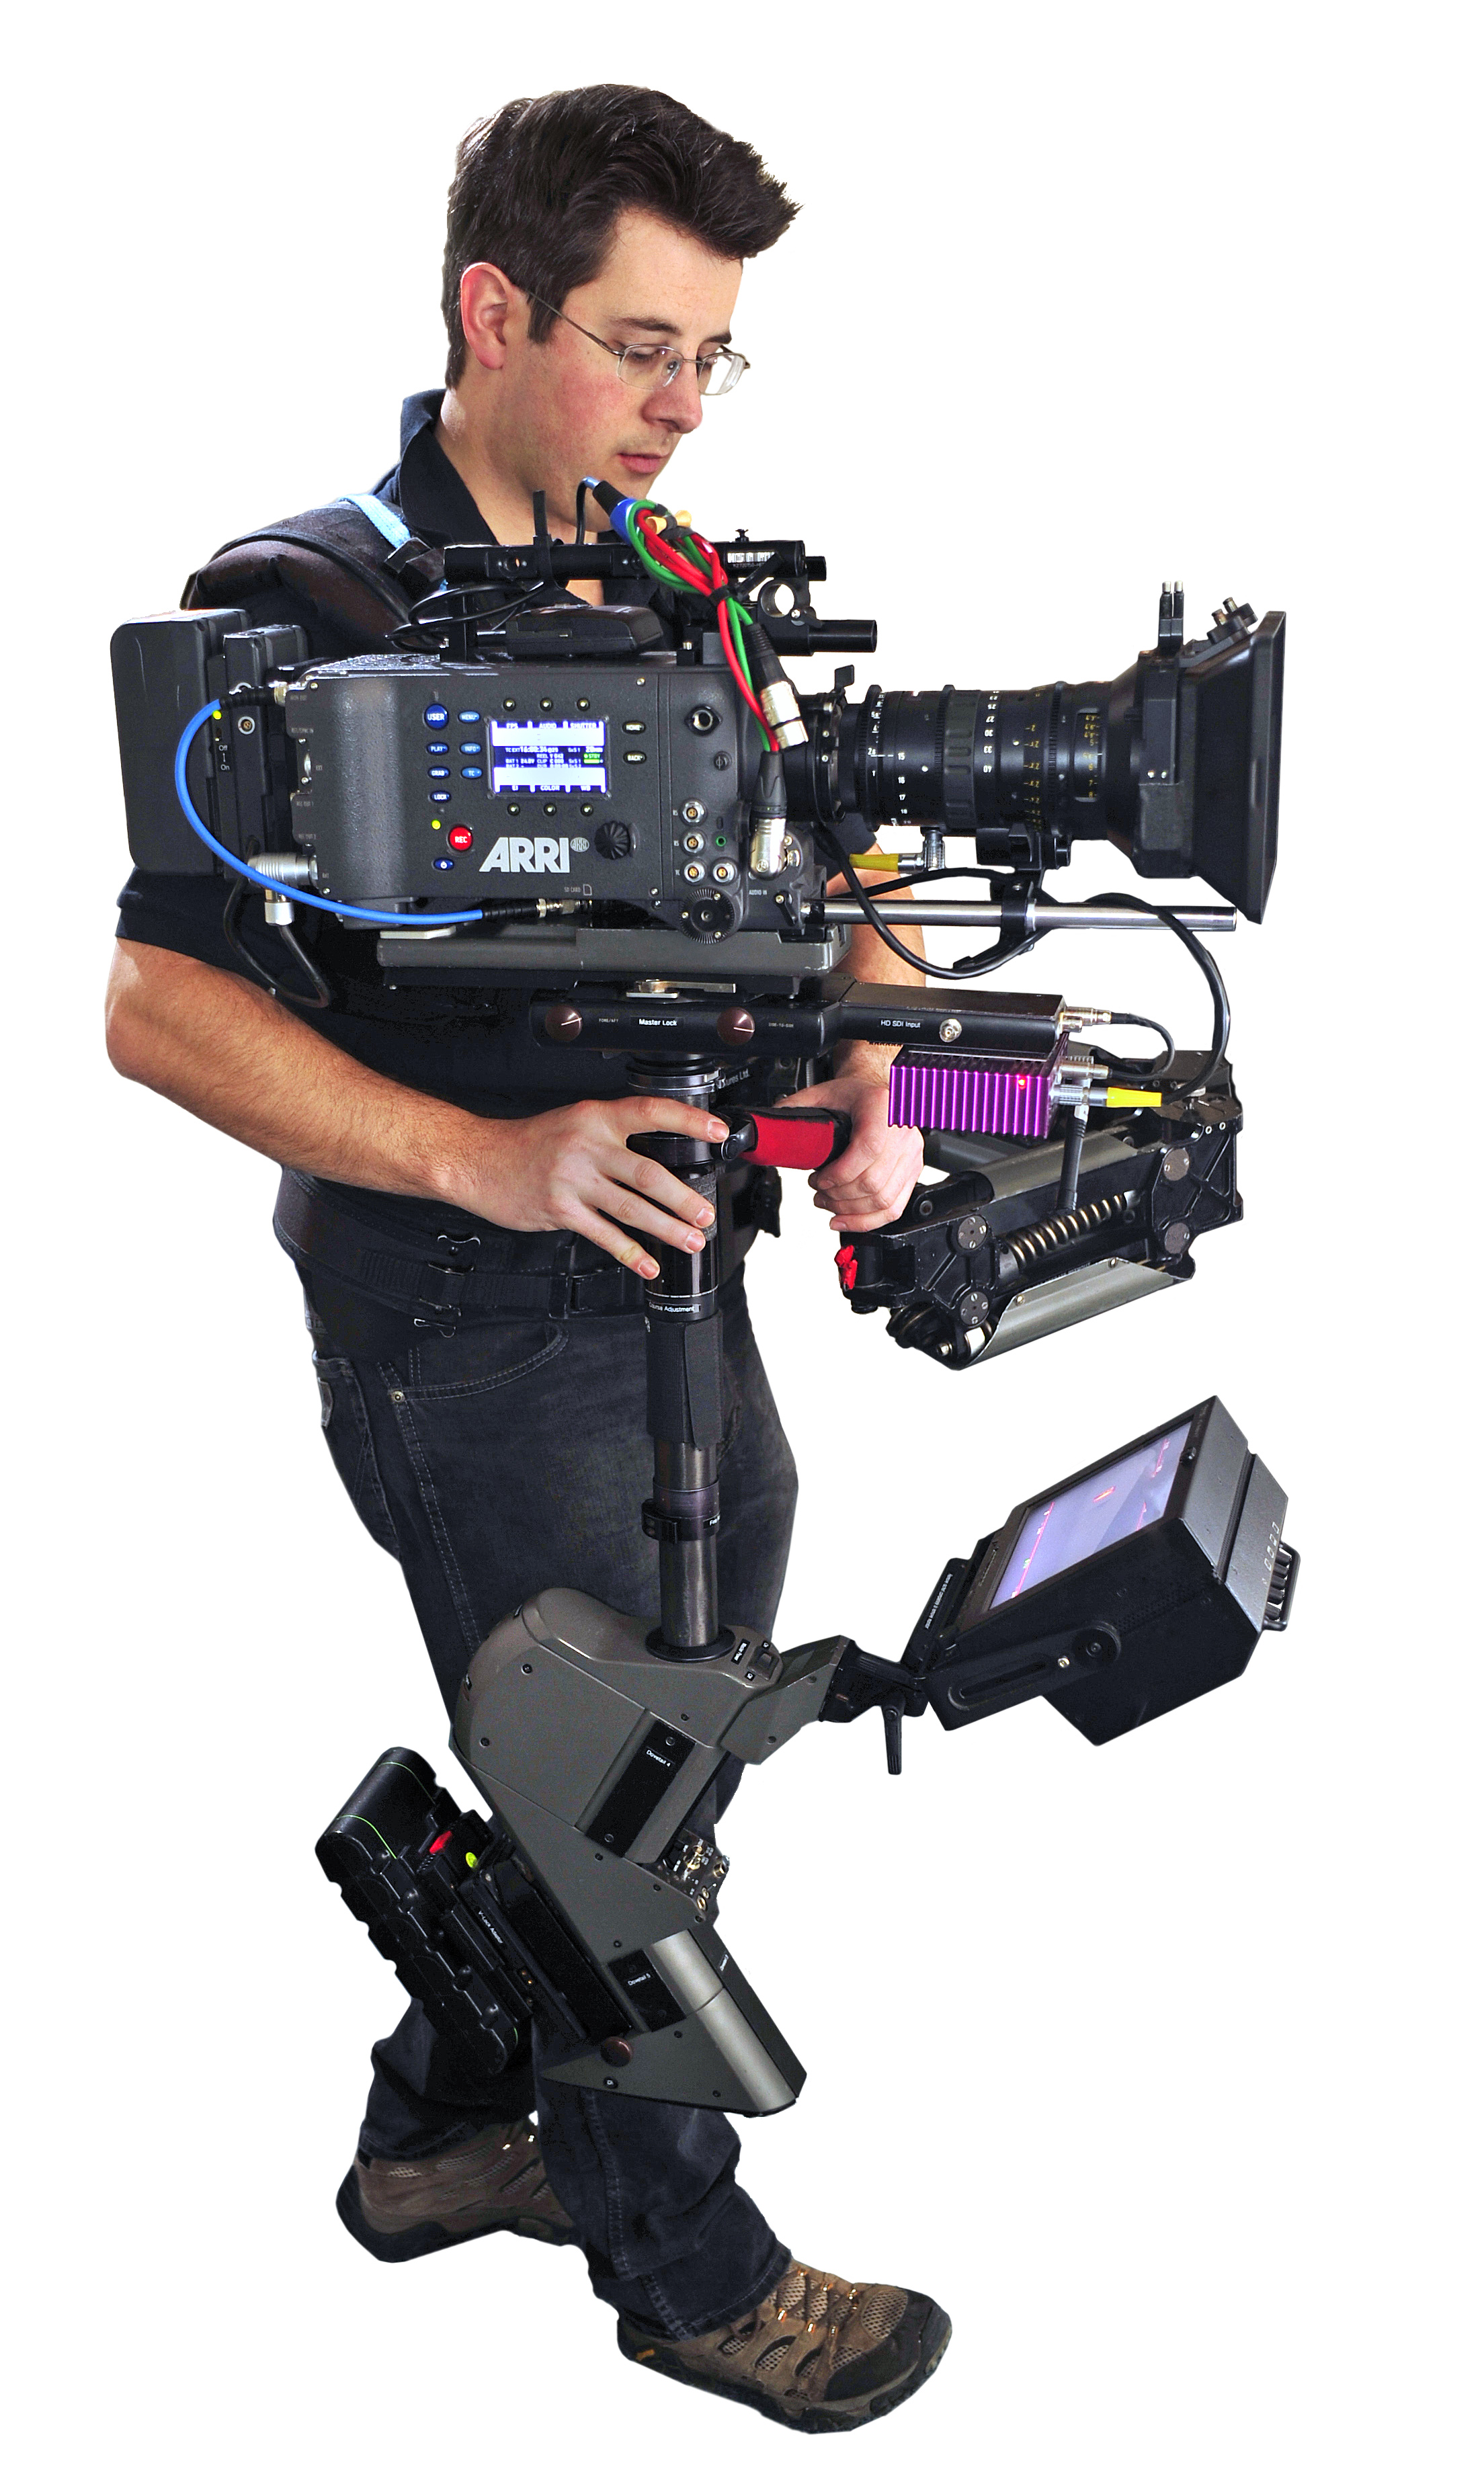
\includegraphics[width=2.0 in]{figuras/camera.jpg}
%\caption{Ilustração dos processos possíveis na interação entre radiação e matéria.}
\end{figure}
\end{frame}


\begin{frame}
\begin{figure}
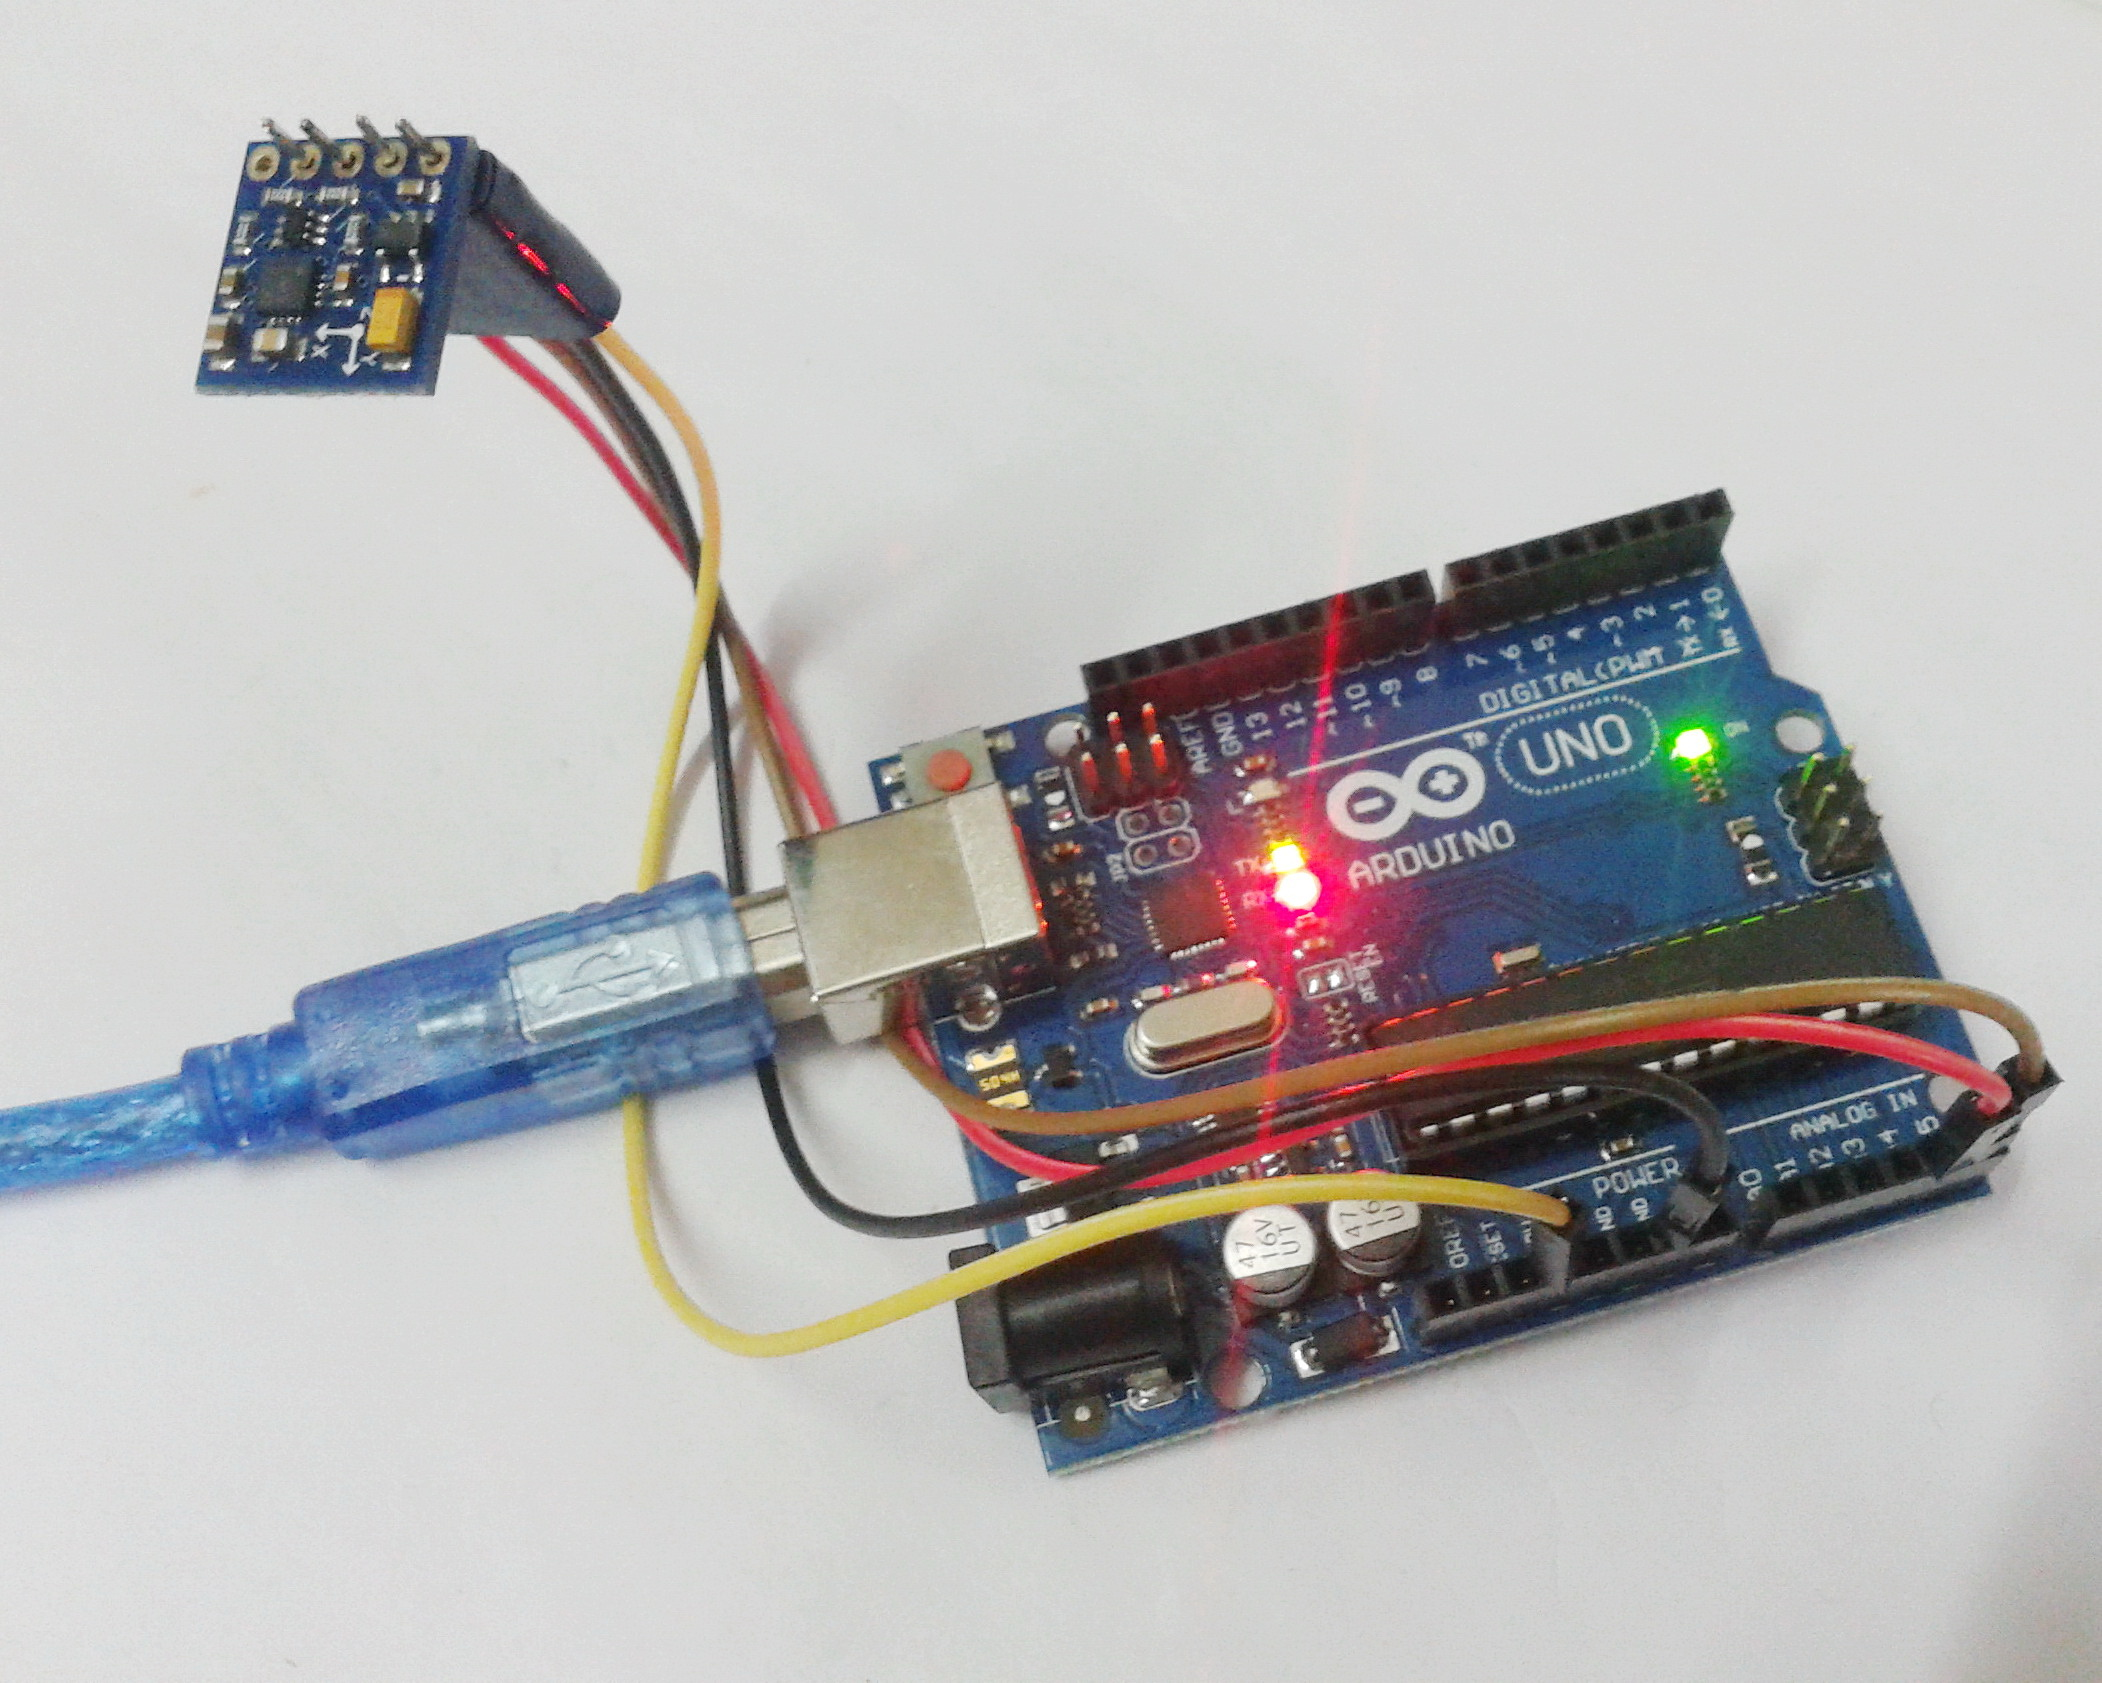
\includegraphics[width=3.5 in]{figuras/Arduino.jpg}
\end{figure}
Micro controlador Arduino acoplado com um sensor giroscópio.
\end{frame}


\begin{frame}
\begin{figure}
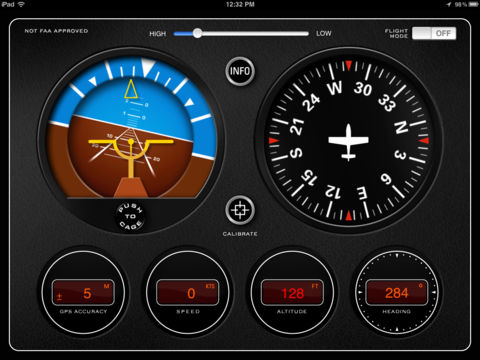
\includegraphics[width=3.5 in]{figuras/aviao.jpg}
\end{figure}
Micro controlador Arduino acoplado com um sensor giroscópio.
\end{frame}



\begin{frame}
\begin{figure}
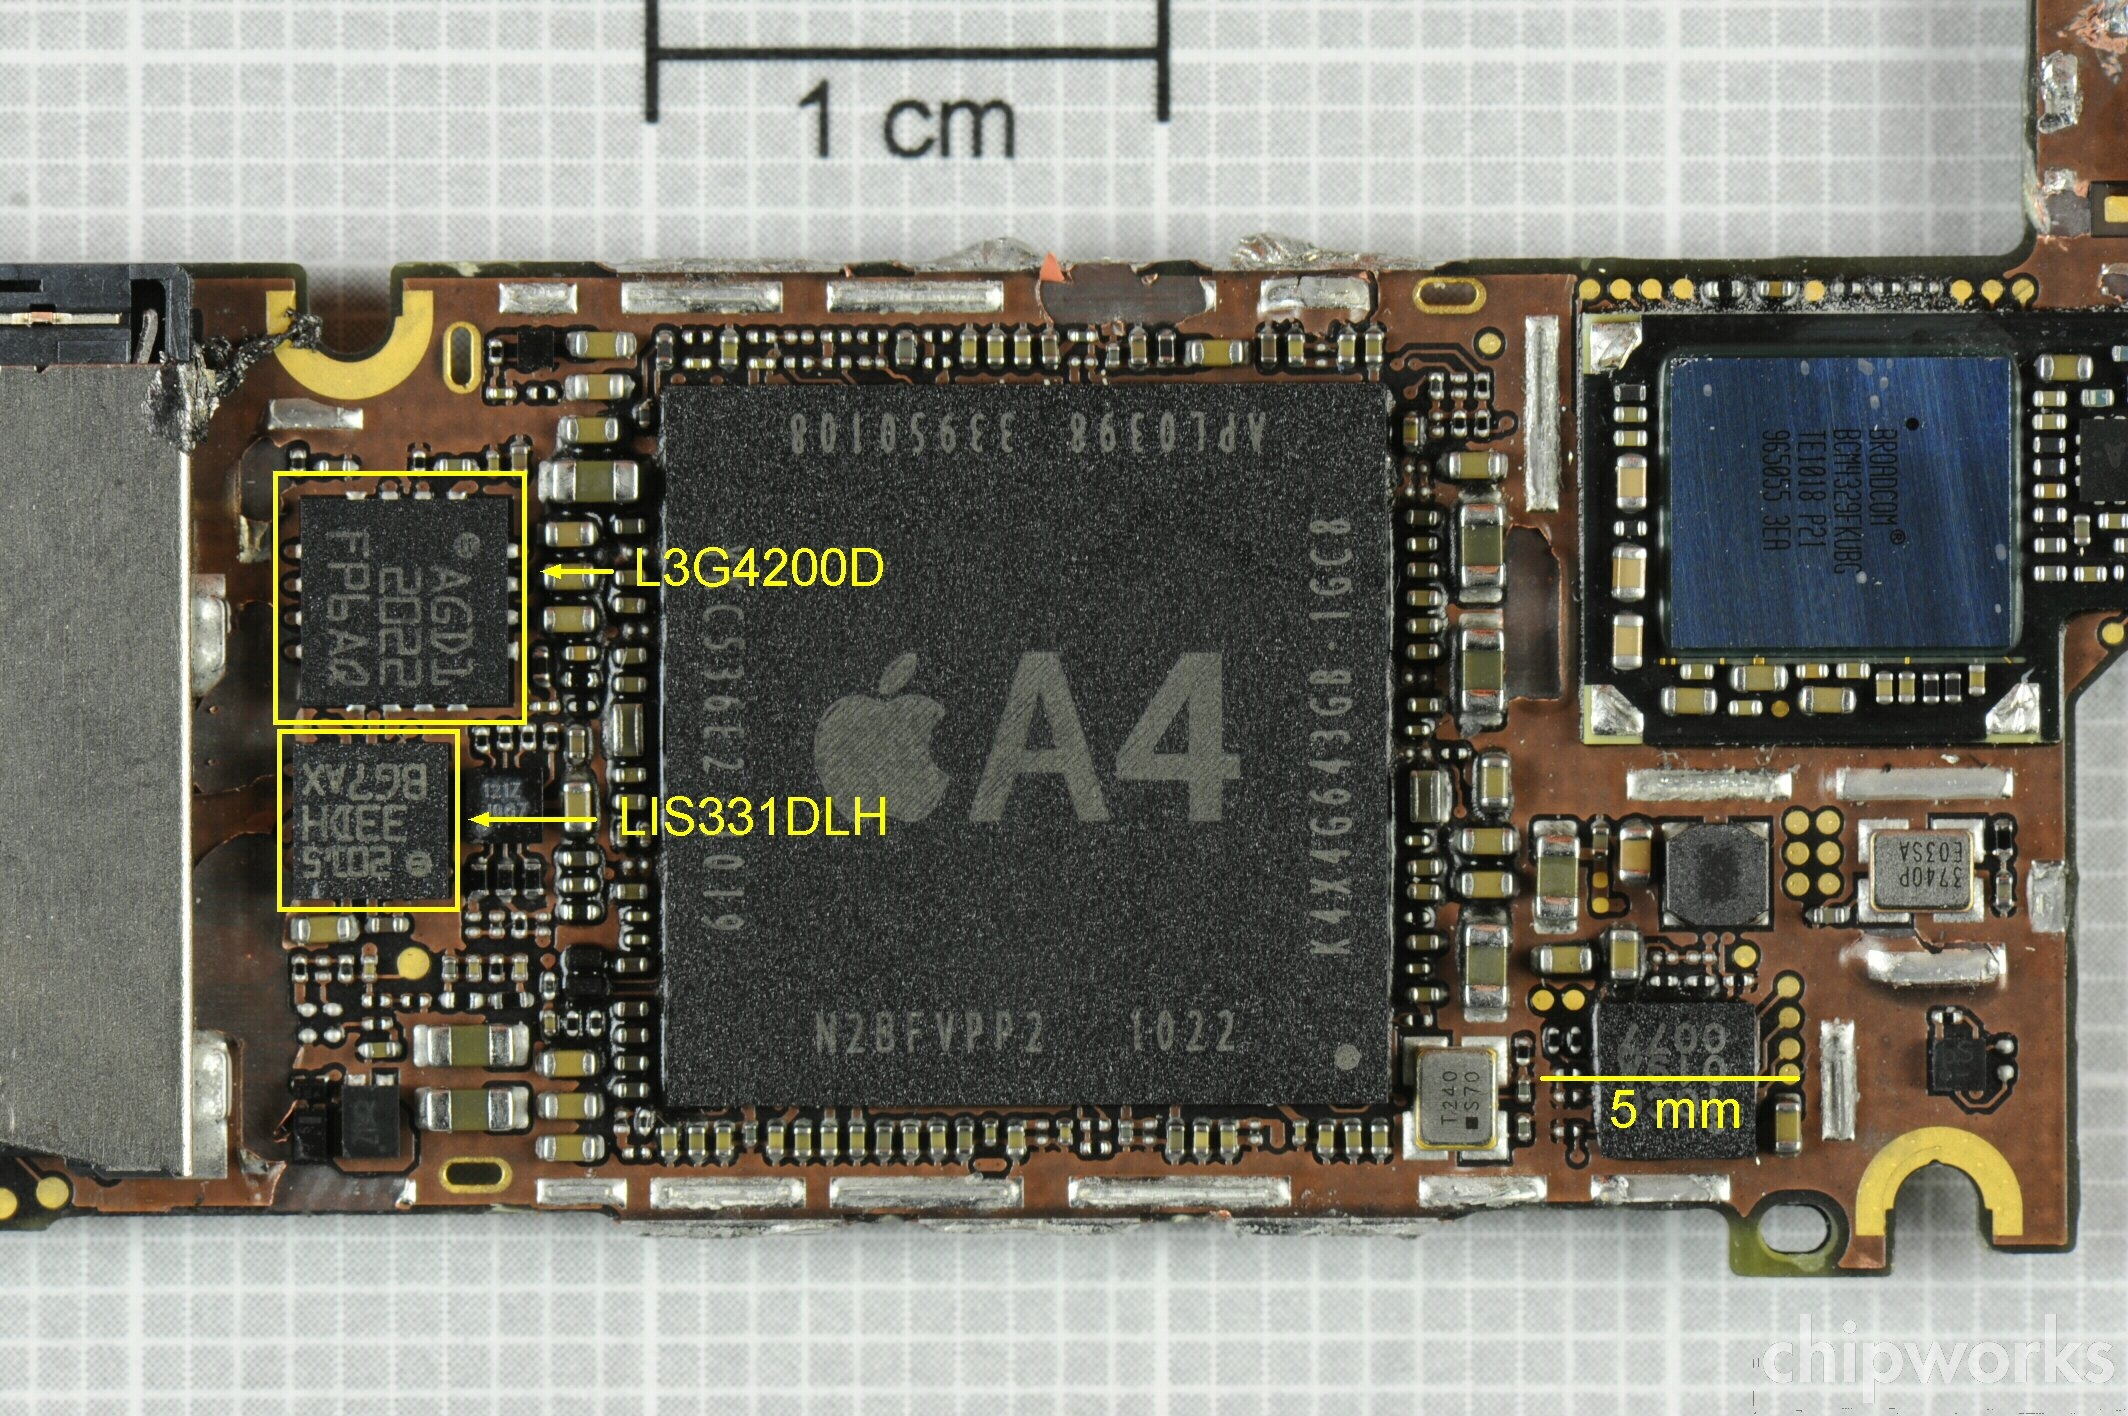
\includegraphics[width=3.7 in]{figuras/giroscopio_iphone.jpg}
\caption{O giroscopio é o L3G4200D.}
\end{figure}
\end{frame}







\begin{thebibliography}{9}

      \begin{frame}[label=bibliography]{Bibliography}
      %\framesubtitle{\TeX, \LaTeX, and Beamer}
      
\bibitem{Serway2014} R. A. Serway, J. W. Jewett, Jr, \textit{Physics: for Scientists and Engineers}, 9th edition Brooks/Cole Cengage Learning 2014.

    \end{frame}
    \end{thebibliography}

\begin{frame}
\Huge{\centerline{Obrigado!}}
\end{frame}

%----------------------------------------------------------------------------------------

%%%%%%%%%%%%%%%%%%%%%%%%%%%%%%%%%%%%%%%%%%%%%%%%%%
% comment out all the contents of the former file
\fi
%%%%%%%%%%%%%%%%%%%%%%%%%%%%%%%%%%%%%%%%%%%%%%%%%%

\end{document}